%%%%%%%%%%%%%%%%%%%%%%%%%%%%%%%%%%%%%%%%%%%%%%%%%%%%%%%%%
%       KAPITOLA 1 - Úvod
%%%%%%%%%%%%%%%%%%%%%%%%%%%%%%%%%%%%%%%%%%%%%%%%%%%%%%%%%
\chapter{Úvod}
\label{kapitola:uvod}
Neuronové sítě (anglicky neural networks) mají v~dnešním světě mnoho využití. Jelikož se jedná o~jednu z~aplikací umělé inteligence (anglicky artificial intelligence), lze neuronové sítě použít například k~rozpoznávání řeči, zpracování přirozeného jazyka či k~detekci obličejů.
Tyto činnosti jsou pro běžného člověka poměrně snadné, avšak pro počítače znamenají relativně náročnou činnost.

Lidé jsou schopni velmi dobře rozeznat obličeje jiných lidí, bez ohledu na světelné podmínky, úhel natočení či částečné zakrytí tváře. Počítačové algoritmy a neuronové sítě zaměřující se na detekci obličejů v~těchto neideálních podmínkách musí být těmto jevů přizpůsobeny.

Aby byly počítače schopné tyto akce vykonávat v~rozumném čase (případně v~reálném čase), je potřeba, aby neuronové sítě byly dostatečně rychlé. Zrychlení neuronové sítě lze dosáhnout buď optimalizací kódu, vylepšením procesu trénování neuronové sítě nebo také využitím speciálních hardwarových zařízení. 

Tato práce se zabývá problematikou výše zmíněných fenoménů, konkrétně optimalizací a zrychlením neuronových sítí pro detekci obličejů v~neoptimálních světelných podmínkách. Z~oblasti neuronových sítí byly použity konvoluční neuronové sítě, k~jejichž trénování je využito jak dat z~běžných datasetů tváří, tak dat ze specializovaných datasetů obličejů a osob ve špatném osvětlení. 

O~akceleraci neuronové sítě se stará zařízení Intel Neural Compute Stick 2 (NCS2) s~knihovnou OpenVINO. V~práci jsou také zmíněny dostupné komerční a nekomerční systémy a řešení pro detekci obličejů.

V~rámci kapitoly \ref{kapitola:detekce_obliceje} je popsána problematika detekce obličeje v~reálných podmínkách, včetně problémů, které detekci ztěžují či přímo znemožňují. Tato část také popisuje klasické přístupy k~detekci obličejů jako jsou algoritmy Viola--Jones nebo Local Binary Patterns.

Kapitola \ref{kapitola:neuronove_site} se věnuje neuronovým sítím jak obecně (perceptron, aktivační funkce, učení), tak konkrétně konvolučním neuronovým sítím. Dále jsou v~kapitole popsány datasety pro učení neuronových sítí a existující řešení detekce obličeje založené na neuronových sítích (YOLO, MTCNN, SSD), včetně jejich porovnání a porovnání algoritmů zaměřených na detekci ve špatných světelných podmínkách.

Popis používaných řešení a systémů k~detekci a popis akcelerace detekčních algoritmů tvoří obsah kapitoly \ref{kapitola:kamery_a_systemy}. Konkrétně je zde popsáno zařízení NCS2.



%%%%%%%%%%%%%%%%%%%%%%%%%%%%%%%%%%%%%%%%%%%%%%%%%%%%%%%%%
%       KAPITOLA 2 - Detekce obličejů
%%%%%%%%%%%%%%%%%%%%%%%%%%%%%%%%%%%%%%%%%%%%%%%%%%%%%%%%%
\chapter{Detekce obličeje v~reálných podmínkách}
\label{kapitola:detekce_obliceje}
Detekce obličeje (anglicky face detection) \cite{fdReview, frReview} je technologie, která umožňuje v~digitálním obrázku lokalizovat lidský obličej. Detekce obličeje patří do skupiny technologií HCI (Human--Computer interaction).
Detekovat obličej je poměrně jednoduchý úkol pro lidi, ale zároveň se jedná o~relativně náročný úkol pro počítače.
Detekce obličeje je výchozím bodem pro další algoritmy analyzující lidský obličej, jako je například (v~závorce za pojmem následuje anglický výraz):
\begin{itemize}
  \item rozpoznávání obličeje (face recognition),
  \item zarovnání obličeje (face alignment),
  \item autentizace pomocí obličeje (face verification/authentication),
  \item sledování pohybu hlavy (head pose tracking),
  \item určování věku nebo pohlaví (age/gender recognition),
  \item[] a mnoho dalších. 
\end{itemize}

Samotná detekce obličeje se v~realném prostředí využívá například v~oblasti fotografování (automatické ostření na tvář), marketingu (zjišťování zájmu zákazníku o~produkty podle počtu výskytu obličejů) nebo bezpečnosti (bezpečnostní kamery a systémy).

Následující podkapitoly se zabývají principem fungování detekce obličeje v~reálných podmínkách a problémy a omezeními, které se v~běžném světě vyskytují a detekce by si s~nimi měla umět poradit (špatné světelné podmínky, příliš členité pozadí, přílišný počet obličejů v~obrázku, barva kůže, nízké rozlišení atd.). Na konci této kapitoly se nachází popis algoritmů a detektorů, které k~detekci přímým způsobem nepoužívají neuronové sítě.

\begin{figure}[H]
  \begin{center}
      \scalebox{0.31}{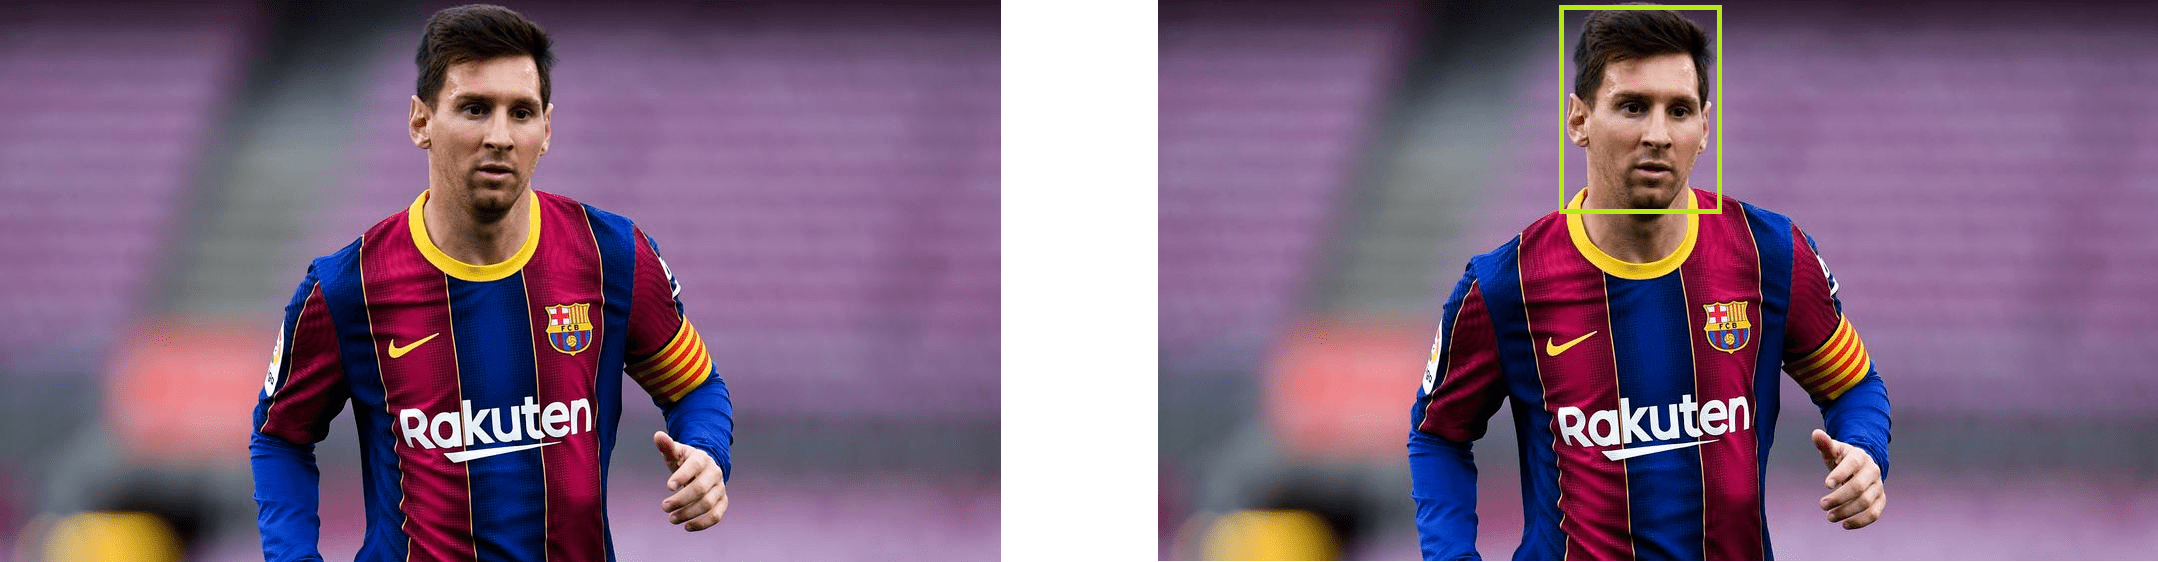
\includegraphics{obrazky-figures/fdexample.png}}
  \label{fdexample}
  \caption{Příklad detekce obličeje}
  \end{center}
\end{figure}

\section{Detekce obličeje}
Způsoby detekce obličeje lze rozdělit do několika skupin, vědecké práce na toto téma se liší a nelze jasně říci zda to či ono dělení je jediné korektní.

Dle \cite{fdReview} existují 2 různé přístupy k~hledání tváří v~obrázcích, a to \textbf{přístup založený na vlastnostech} (anglicky feature based approach) a \textbf{přístup založený na obrázku} (anglicky image based approach). 
\textbf{Přístup založený na vlastnostech} nepoužívá přímo k~detekci obličeje neuronové sítě. Využívá vlastností obličeje jako takového (rysy, pozice očí, uší, obočí, barva kůže\dots). Efektivita tohoto přístupu se snižuje s~výskyty problémů popsaných v~sekci \ref{sekce:problemy}, protože může docházet například k~zakrytí nebo špatné viditelnosti některých vlastností obličeje.

Naproti tomu \textbf{obrazový přístup} uplatňuje schopnosti neuronových sítí a umělé inteligence k~natrénování modelu neuronové sítě a následné přímé detekci pomocí tohoto modelu. 

Podle \cite{feature-based-fd-review} lze rozdělit metody detekce obličeje do 4 základních kategorií (viz obrázek \ref{fddeleni}) a 2 zvláštních kategorií (Haarovy vlastnosti a umělá inteligence).
\begin{figure}[H]
  \begin{center}
      \scalebox{0.9}{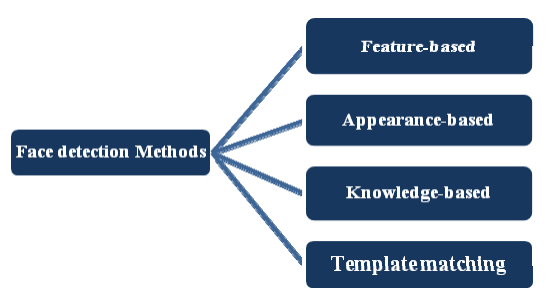
\includegraphics{obrazky-figures/fddeleni.png}}
  \label{fddeleni}
  \caption{Dělení metod detekce obličeje dle \cite{feature-based-fd-review}}
  \end{center}
\end{figure}

\textbf{Feature-based methods} (metody založené na vlastnostech) opět pracují s~vlastnostmi obličeje. Vyhledávají v~obraze rysy obličeje. Detekci může výrazně ztížit či znemožnit neviditelnost některých rysů. Výhodou těchto metod je rychlost v~porovnání s~ostatními metodami.

\textbf{Appearance-based methods} (metody založené na vzhledu/obrázku) využívají klasifikace vlastností tváře do 2 tříd v~podobrázku celého obrázku. Klasifikátory podle nichž se daná metoda rozhoduje, zda se jedná o~tvář či nikoli, mají různé váhy, metoda postupuje od slabých klasifikátorů k~silnějším.

Metody založené na znalostech (\textbf{Knowledge-based mathods}) se uplatňují při detekci obličeje v~obrázku s~členitým/komplexním pozadím. Znalosti, které k~detekci pomáhají jsou například: obličej má 2 uši, jeden nos, jedny ústa nebo známé vzdálenosti mezi jednotlivými rysy obličeje.

\textbf{Templatematching} (šablonování, maskování) aplikuje na obrázek předem danou ma-sku obličeje a snaží se detekovat obličej pomocí postupného maskování. Tato metoda je snadná na implementaci, jejím nedostatkem je však závislost na přímém pohledu tváře na obrázku.

Haarovými vlastnostmi a neuronovými sítěmi se zabývají sekce \ref{sekce:viola_jones}, respektive \ref{sekce:NS}.

\section{Problémy a omezení}
\label{sekce:problemy}
Algoritmy pro detekci obličejů čelí několika výzvám a omezením spojených s~ne vždy perfektním zobrazením obličeje v~obrázku. Lidské obličeje na fotografiích a obrázcích mohou být částečně zakryté (např. sluneční brýle), fotografie mohou být pořízené za nevhodných světelných podmínek (např. zastínění části tváře) nebo mohou obrázky nabývat nedostatečné kvality (nízké rozlišení).

Jelikož tedy vstupní obrázek detekce obličeje nemusí být vždy ideální, nemusí být obličej vždy správně detekován.
V~této sekci jsou popsány některé problémy \cite{feature-based-fd-review, fdReview}, které mohou bránit v~úspěšné detekci. Minimalizace dopadu těchto jevů na detekci je klíčem k~navýšení uspěšnosti detekce. Mezi problémy a omezení (viz obrázek \ref{fdproblems}) pro detekci patří pozice hlavy, zakrytí části/částí obličeje, špatně osvětlená scéna nebo výraz tváře.

\begin{figure}[H]
  \begin{center}
      \scalebox{0.5}{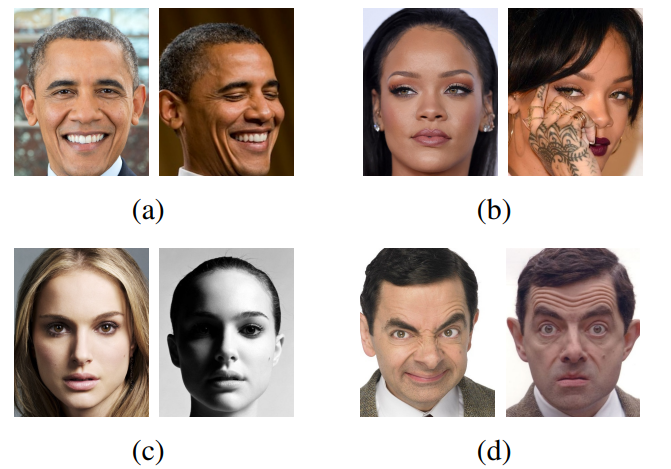
\includegraphics{obrazky-figures/fdproblems.png}}
  \label{fdproblems}
  \caption{Vybráné problémy při detekci obličejů \cite{frReview}. (a) Pozice hlavy; (b)~Zakrytí části obličeje; (c) Špatné světelné podmínky; (d) Výraz tváře}
  \end{center}
\end{figure}

\subsection*{Pozice hlavy}
Hlava může být na fotografii různě natočena, takže obličej nemusí být zachycen v~přímém pohledu do kamery, ale může být zaznamenán z~profilu nebo ze šikma (poloprofil) jako na obrázku \ref{fdproblems} část (a).

\subsection*{Zakrytí části obličeje}
Výsledek detekce může být ovlivněn i zakrytím části obličeje (rukou, brýlemi, vlasy, šátkem apod.).

\subsection*{Výraz tváře}
Výraz lidského obličeje mohou ovlivnit emoce a nálady. Detektor \cite{emotionDetector} zabývající se detekcí a rozpoznáváním emocí dosahuje přesnosti 96 \%.

\subsection*{Orientace obrázku}
Problémem pro detekci může být různá orientace obrázku (vzhůru nohama, zrcadlově otočený, natočený do strany apod.). Na obrázek je tak nutno aplikovat některé tranformační operace pro zarovnání.


\subsection*{Nedostatečně výkonná detekce}
Velmi důležitým faktorem při detekci obličejů, zvláště v~real-timových aplikacích, je rychlost detekce. Pokud má algoritmu vysokou přesnost, ale je příliš pomalý pro vybranou aplikaci, stává se nepoužitelným. Akcelerací detekčních algoritmů se mj. zabývá i tato práce.

\subsection*{Příliš členité pozadí} 
Pokud se v~o~brázku nachází příliš mnoho objektů, může dojít ke snížení přesnosti a rychlosti detekce.

\subsection*{Přílišný počet obličejů v~obrázku}
Výskyt velkého počtu obličejů v~jednom obrázku, často překrývajících se, může představovat výzvu pro detekční algoritmus. 

\subsection*{Nízké rozlišení}
Obrázky a fotografie s~nízkým rozlišením nemusejí obsahovat dostatek informace nutné ke správnemu detekování tváře.

\subsection*{Špatné světelné podmínky}
Na detekci mohou mít vliv světelné podmínky panující při pořizování zkoumané fotografie či videa. Aspekty jež světlo ovlivňuje jsou mj. jas, kontrast, barvy, stíny, ostrost. Tato práce se zabývá detekcí obličejů v~záznamech, v~nichž některý z~těchto faktorů omezuje detekci.


\begin{figure}[H]
  \begin{center}
      \scalebox{0.8}{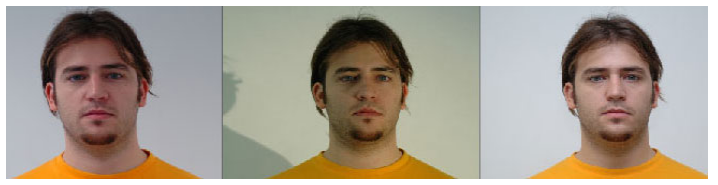
\includegraphics{obrazky-figures/illuminationexample.png}}
  \label{illuminationexample}
  \caption{Příklad stejného obličeje vyfoceného při různých světelných podmínkách \cite{feature-based-fd-review}}
  \end{center}
\end{figure}

\section{Algoritmy detekce obličeje}
\label{sekce:detektory_bez_neuronovych_siti}
Existuje několik různých přístupů k~detekci obličeje. Tato sekce se zaměřuje na detekci s~využitím detektorů založených primárně ne na neuronových sítích (neuronová síť není použita vůbec, nebo není použita k~přímé detekci). Detektory obličeje využívající principy neuronových sítí k~přímé detekci jsou popsány v~sekci \ref{sekce:NSdetektory}.

\subsection*{Local Binary Patterns}
Algoritmus využívající \textbf{lokální binární vzory} (anglicky Local Binary Patterns -- dále jen LBP) pro popis struktury/textury obrázku má mnoho aplikací \cite{localBinaryPatterns}. Jedná se o~jeden z~nejvýkonnějších algoritmů pro popis textur v~obrázcích. LBP algoritmus má vysokou účinnost detekce (89 \%) \cite{localBinaryPatternsTests} a nízkou výpočetní náročnost.
LBP pracuje s~černobílými (anglicky gray--scale) obrázky a v~původní verzi funguje tak, že každému pixelu přiřadí binární číselnou hodnotu, vypočítanou dle hodnot pixelů v~3 $\times$ 3 okolí daného pixelu. Každý takovýto pixel v~okolí je ohodnocen hodnotou buď 1 nebo 0 v~závislosti na tom, zda jeho hodnota překročila stanovený práh (anglicky threshold), kterým je hodnota prostředního pixelu (viz obrázek \ref{lbp}).

\begin{figure}[H]
  \begin{center}
      \scalebox{0.8}{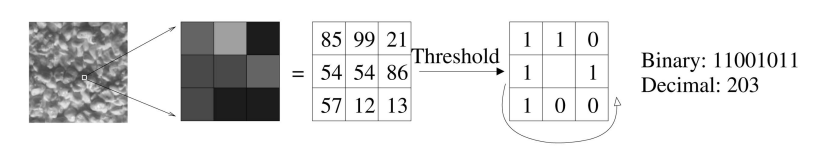
\includegraphics{obrazky-figures/lbp.png}}
  \label{lbp}
  \caption{Ukázka ohodnocení pixelu algoritmem LBP \cite{localBinaryPatterns}}
  \end{center}
\end{figure}

Algoritmus byl později vylepšen tak, aby uměl pracovat s~různě velkým okolím, které navíc nemusí mít čtvercový tvar. Používané okolí ve tvaru kružnice je popsáno dvojicí $(P, R)$, kde $P$ je počet vzorkovacích bodů a $R$ je poloměr kružnice. Další vylepšení LBP algoritmu se týkalo definování tzv. uniformních vzorů (anglicky uniform patterns). Tyto vzory jsou ty vzory v~nichž se vyskytují nejvýše 2 přechody z~1 na 0 a opačně. Příkladem uniformního vzoru na okolí $(8, 2)$ je 11100000 (1 přechod), či 00111000 (2 přechody). 

Lokální primitiva (obrázek \ref{lbpprimitives}) a histogramy vytvořené z~takto získaných hodnot se využívají mj. k~detekci obličejů.

\begin{figure}[H]
  \begin{center}
      \scalebox{0.8}{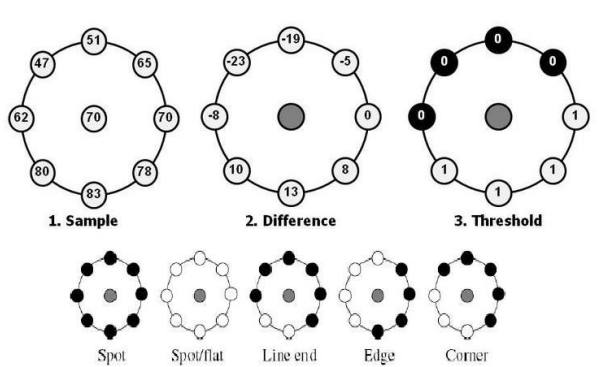
\includegraphics{obrazky-figures/lbpPrimitives.png}}
  \label{lbpprimitives}
  \caption{Lokální primitiva detekované algoritmem LBP \cite{localBinaryPatternsTests}}
  \end{center}
\end{figure}

\subsection*{Viola--Jones algoritmus}
\label{sekce:viola_jones}
Algoritmus \textbf{Viola--Jones} \cite{violaJonesArticle, violaJones}, někdy také nazývaný \textbf{Haar Cascades}, je obecně technika pro detekci objektů, vytvořená před používáním metod hlubokého učení. Používá se k~detekci obličejů, částí těla, očí, úst atd. Dosahuje přesnosti detekce kolem 90 \% \cite{violaJones}. 

Princip fungování algoritmu spočívá v~detekci hran a čár (obecně vlastností) v~černobílém obrázku (hodnoty pixelů jsou na intervalu $<0; 1>$). Vybere se jedna z~vlastností (některé z~nich zobrazuje obrázek \ref{haarfeatures}) a vypočítá se průměrná hodnota pixelů ve všech obdélnících (obdélníky jsou dva, tři nebo čtyři). Rozdíl těchto hodnot pak určuje zda se jedná o~hranu, čáru tzn. zda je daná vlastnost detekována. Pokud například budeme hledat vlastnost \emph{b)} z~obrázku \ref{haarfeatures} a vypočtený rozdíl hodnot je blízký 1, detekce byla úspěšná (viz ukázka v~obrázku \ref{haarexample}).

\begin{figure}[H]
  \begin{center}
      \scalebox{0.6}{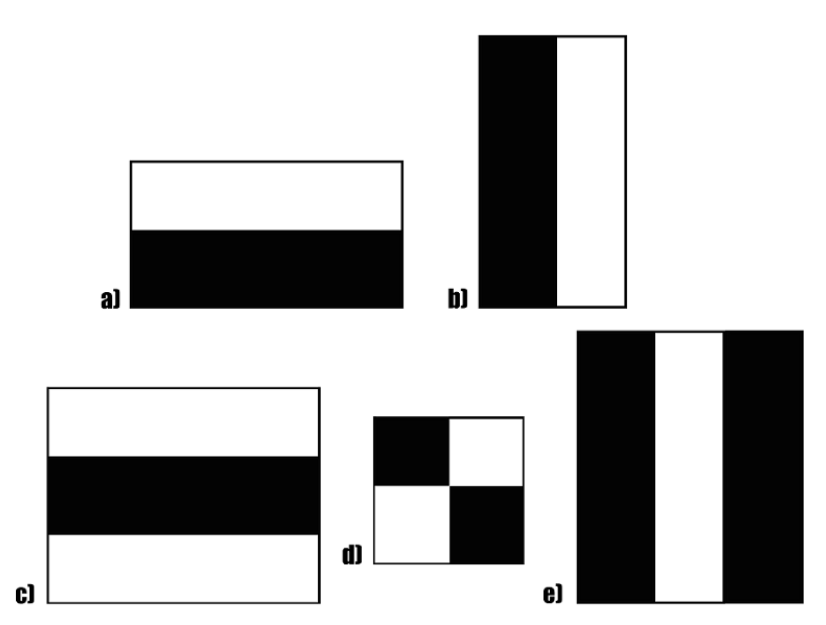
\includegraphics{obrazky-figures/haarfeatures.png}}
  \label{haarfeatures}
  \caption{Haarovy vlastnosti \cite{violaJonesArticle}
  a) horizontální hrana; b) horizontální hrana; c) horizontální čára d) diagonála e) vertikální čára}
  \end{center}
\end{figure}

\begin{figure}[H]
  \begin{center}
      \scalebox{0.4}{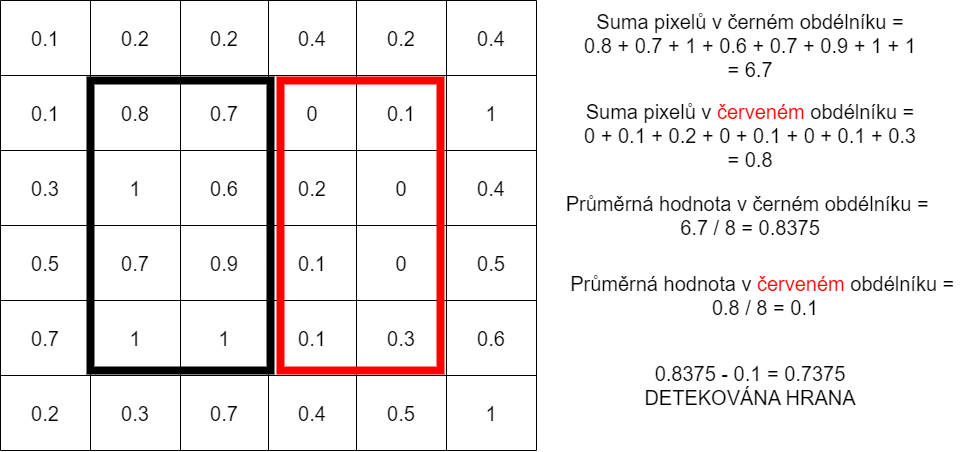
\includegraphics{obrazky-figures/haarexample.png}}
  \label{haarexample}
  \caption{Příklad výpočtu detekce hrany dle vlastnosti b) z~obrázku \ref{haarfeatures}. Bílý obdélník je nahrazen červeným pro lepší viditelnost.}
  \end{center}
\end{figure}

Algoritmus postupně prochází celý obrázek a hledá výskyt některé z~vlastností. Toto procházení u~obrázků s~velkým počtem pixelů znamená enormní výpočetní nároky, protože je potřeba vždy počítat s~hodnotami všech dotčených pixelů. Proto Viola a Jones \cite{violaJones} navrli
vylepšení nazvané anglicky \textbf{Integral Image}. To spočívá v~tom, že všechny pixely stačí projít pouze 1x, a každý tento pixel lze ohodnotit sumou hodnot pixelů směrem nalevo a nahoru (důsledkem je, že pixel s~nejnižším ohodnocení se nachází v~levém horním rohu a pixel s~nejvyšším ohodnocením v~pravém dolním rohu). Následný výpočet průměrné hodnoty ukazuje obrázek \ref{integralimage}. 

\begin{figure}[H]
  \begin{center}
      \scalebox{0.7}{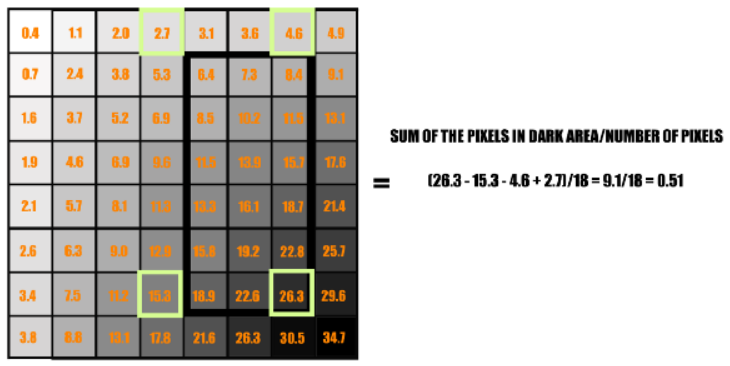
\includegraphics{obrazky-figures/integralimage.png}}
  \label{integralimage}
  \caption{Ukázka výpočtu hodnoty obdélníku v~Haarově vlastnosti za pomoci vylepšení \textbf{Integral Image} \cite{violaJonesArticle}.}
  \end{center}
\end{figure}

Jelikož Haarových vlastností je velké množství, bylo vybráno 6000 nejvíce vyhovujících, které se k~detekci obličejů používají. Detekce je rozdělena na několik etap, v~každé etapě je vyhledáván v~části obrázku výskyt několika vlastností (počet s~každou etapou roste), pokud se vyhledání nezdaří, není již dále daná část obrázku prohledávána. 


\subsection*{Histogram orientací gradientů}
Metoda HOG (anglicky Histograms of Oriented Gradients) \cite{hog, hog2} používá k~detekci obličejů či postav histogramy orientovaných přechodů v~obrázku, rozděleném dle mřížky na několik bloků (často například 8$\times$8 nebo 4$\times$4 pixelů). Pro každý pixel v~takovémto bloku jsou vypočítány hodnoty gradientů -- velikost (magnitude) a směr (direction). Tyto hodnoty jsou pak přiřazeny do jednoho či více sloupců v~histogramu popisujícím celý blok.

Tento histogram bývá rozdělen na 9 sloupců (rozmezí -- anglicky bin) vyjadřujících směr gradientu v~úhlu na škále od 0$^\circ$ do 180$^\circ$, kdy každý sloupec odpovídá intervalu 20$^\circ$. Výslednému vektoru, který udává velikosti gradientů v~jednotlivých úhlech se říká HOG deskriptor.

HOG využívá pro zlepšení detekce při zhoršených světelných podmínkách normalizaci HOG deskriptorů. Tato normalizace je prováděna na vektorech 4 sousedících bloků. Pokud je tedy vektor složen z~9 hodnot, vypočítá se normalizační vektor z~$9 \times 4 = 36$ hodnot.

Výsledkem metody je obrázek (viz obrázek \ref{hogexample} reprezentovaný orientovanými gradienty, který se využívá k~detekci osoby nebo obličeje.

\begin{figure}[H]
  \begin{center}
      \scalebox{0.5}{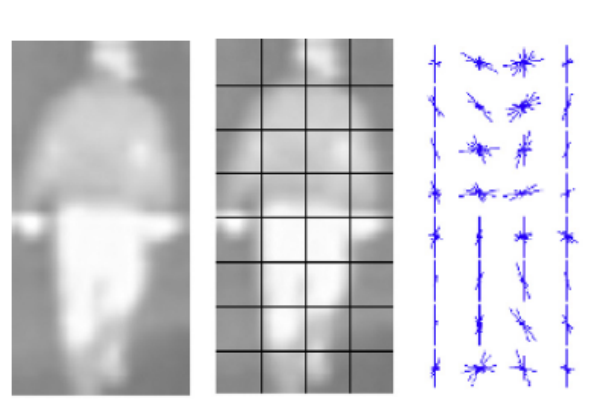
\includegraphics{obrazky-figures/hogexample.png}}
  \label{hogexample}
  \caption{Zleva výřez originálního obrázku převedený do šedotónové reprezentace, rozdělený obrázek na bloky, výstup metody HOG \cite{hog2}.}
  \end{center}
\end{figure}


%%%%%%%%%%%%%%%%%%%%%%%%%%%%%%%%%%%%%%%%%%%%%%%%%%%%%%%%%
%       KAPITOLA 3 - Neuronové sítě
%%%%%%%%%%%%%%%%%%%%%%%%%%%%%%%%%%%%%%%%%%%%%%%%%%%%%%%%%
\chapter{Neuronové sítě pro detekci obličeje}
\label{kapitola:neuronove_site}
Tato kapitola popisuje neuronové sítě a jejich využití pro detekci obličejů. Sekce \ref{sekce:NS} se věnuje popisu neuronových sítí obecně, v~sekci \ref{sekce:datasety} jsou popsány datasety a jejich využití k~trénování neuronových sítí. Sekce \ref{sekce:NSdetektory} se zabývá konkrétními detektory obličejů s~využitím neuronových sítí. Konkrétní programovací frameworky pro práci s~neuronovými sítěmi vyobrazuje sekce \ref{sekce:frameworky_pro_ns}.

\section{Neuronové sítě}
\label{sekce:NS}

Neuronové sítě \cite{deeplearningbook, ns1994} umožňují nalezení neznámého řešení problému pomocí naučení se z~podobných problémů u~nichž známe řešení. Tyto umělé sítě jsou inspirovány biologickou nervovou soustavou lidí (lidským mozkem). Síla neuronových sítí se projevuje v~úlohách zaměřených na detekci, rozpoznávání (objektů, lidí, obličejů, obecně vzorů -- anglicky patterns) a~zpracování dat. Existuje řada druhů neuronových sítí (konvoluční, hluboké, dopředné, rekurentní), pro detekci obličejů v~obrázcích se nejčastěji používají konvoluční neuronové sítě (anglicky Convolutional Neural Networks -- CNN). 

Na princip fungování neuronových sítí může být nahlíženo jako na nelineární matematickou funkci, která převádí $X$ vstupů na $Y$ výstupů. Proces transformace vstupních informací na výstup je ovlivňován váhováním hodnot vně sítě. Tyto hodnoty vah jsou určovány při tzv. učení/trénování neuronových sítí. Pro správné natrénování neuronové sítě je potřeba dostatečného počtu vstupních trénovacích dat (obrázků, textů, hodnot) a~dostatečně výkonný hardware. 

\subsection*{Biologický neuron}
Jak již bylo zmíněno, inspirací neuronových sítí je biologická nervová soustava. V~lidském mozku se nachází okolo $10^{11}$ neuronů (elektricky aktivních buněk spracovávajích signály). Vstupem těchto neuronů jsou tzv. dendrity, výstupy pak nazýváme axony. Jednotlivé neurony jsou navzájem propojeny tisíci spoji pojmenovanými synapse. Synapse zajišťují komunikaci mezi neurony.

Takto vytvořený paralelismus poskytuje mozku schopnost rychle zpracovávat informace. Neurony biologické i umělé pracují s~váhovanými vstupy. Po překročení určitého prahu na vstupech je adekvátně upraven výstup neuronu. Klíčovou vlastností potom je způsobilost měnit hodnoty jednotlivých vah na základě externích vlivů. Tím dochází k~učení sítě neuronů.

\subsection*{Perceptron}

Nejjednoduším modelem umělého neuronu je preceptron. Perceptron má $N$ vstupů, jejichž hodnoty $x$ jsou vynásobeny váhami $w$ a sesumovány dle vzorce \ref{vzorec:perceptron}.

\begin{equation} \label{vzorec:perceptron}
  a = \sum_{i=1}^{N} (w_i * x_i) + w_0 * x_0
\end{equation}

Hodnota $x_0$ se nazývá bias a jedná se o~neměnnou vstupní hodnotu (často má hodnotu $+1$). Váhy a vstupy (včetně biasu) mohou být jak kladné, tak i záporné. Hodnota $a$ je po vypočtení předána tzv. \textbf{aktivační funkci}.

\begin{figure}[H]
  \begin{center}
      \scalebox{0.4}{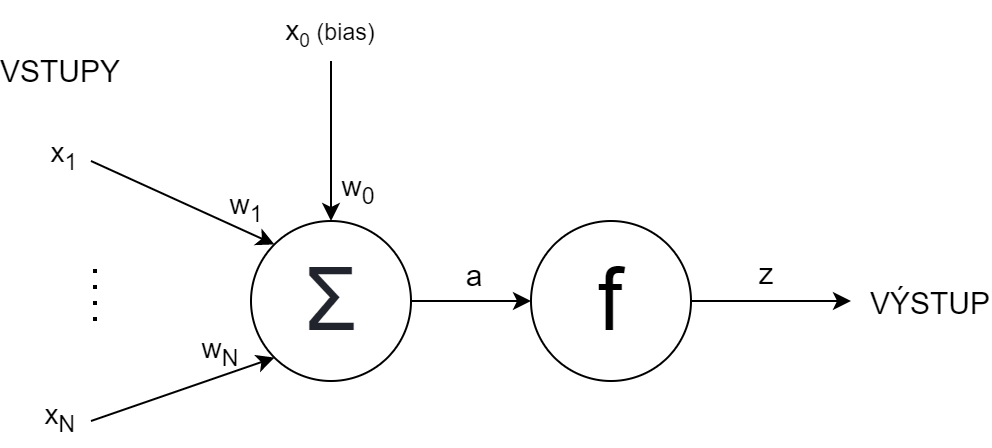
\includegraphics{obrazky-figures/perceptron.png}}
  \label{obrazek:perceptron}
  \caption{Perceptron s~N vstupy, biasem $x_0$ a aktivační funkcí $f$}
  \end{center}
\end{figure}

\subsection*{Aktivační funkce}
Aktivační funkce $f$ je matematická funkce, která určuje výstup neuronu (vzorec \ref{vzorec:aktivacni_fce}). Na výběru vhodné aktivační funkce závisí přesnost neuronové sítě. Funkce může být různá, pro příklad je zde uveden výstup rozlišující zda se jedná o~kladné či záporné číslo nebo nulu (viz vzorec \ref{vzorec:vystup_aktivacni_fce}). V~praxi se často používá aktivační funkce nazvaná \textbf{rectified linear unit} (ReLU) \cite{deeplearningbook} definovaná jako $f(a) = max\{0, a\}$.

\begin{equation} \label{vzorec:aktivacni_fce}
  z~= f(a)
\end{equation}

\begin{equation}
  \label{vzorec:vystup_aktivacni_fce}
   f(a) =
    \begin{cases}
      0       & \quad \text{pro } a = 0\\
      1       & \quad \text{pro } a > 0\\
      -1       & \quad \text{pro } a < 0
    \end{cases}
\end{equation}

\subsection*{Spojování neuronů}
Spojením několika neuronů lze vytvořit tzv. vrstvu (anglicky layer) perceptronů. Tytvo vrstvy se dělí na vstupní (anglicky input), výstupní (anglicky output) a skryté (anglicky hidden). Konkatenací vstupní, několika skrytých a výstupní vrstvy je možno vytvořit neuronovou síť připravenou k~trénování.

\begin{figure}[H]
  \begin{center}
      \scalebox{0.22}{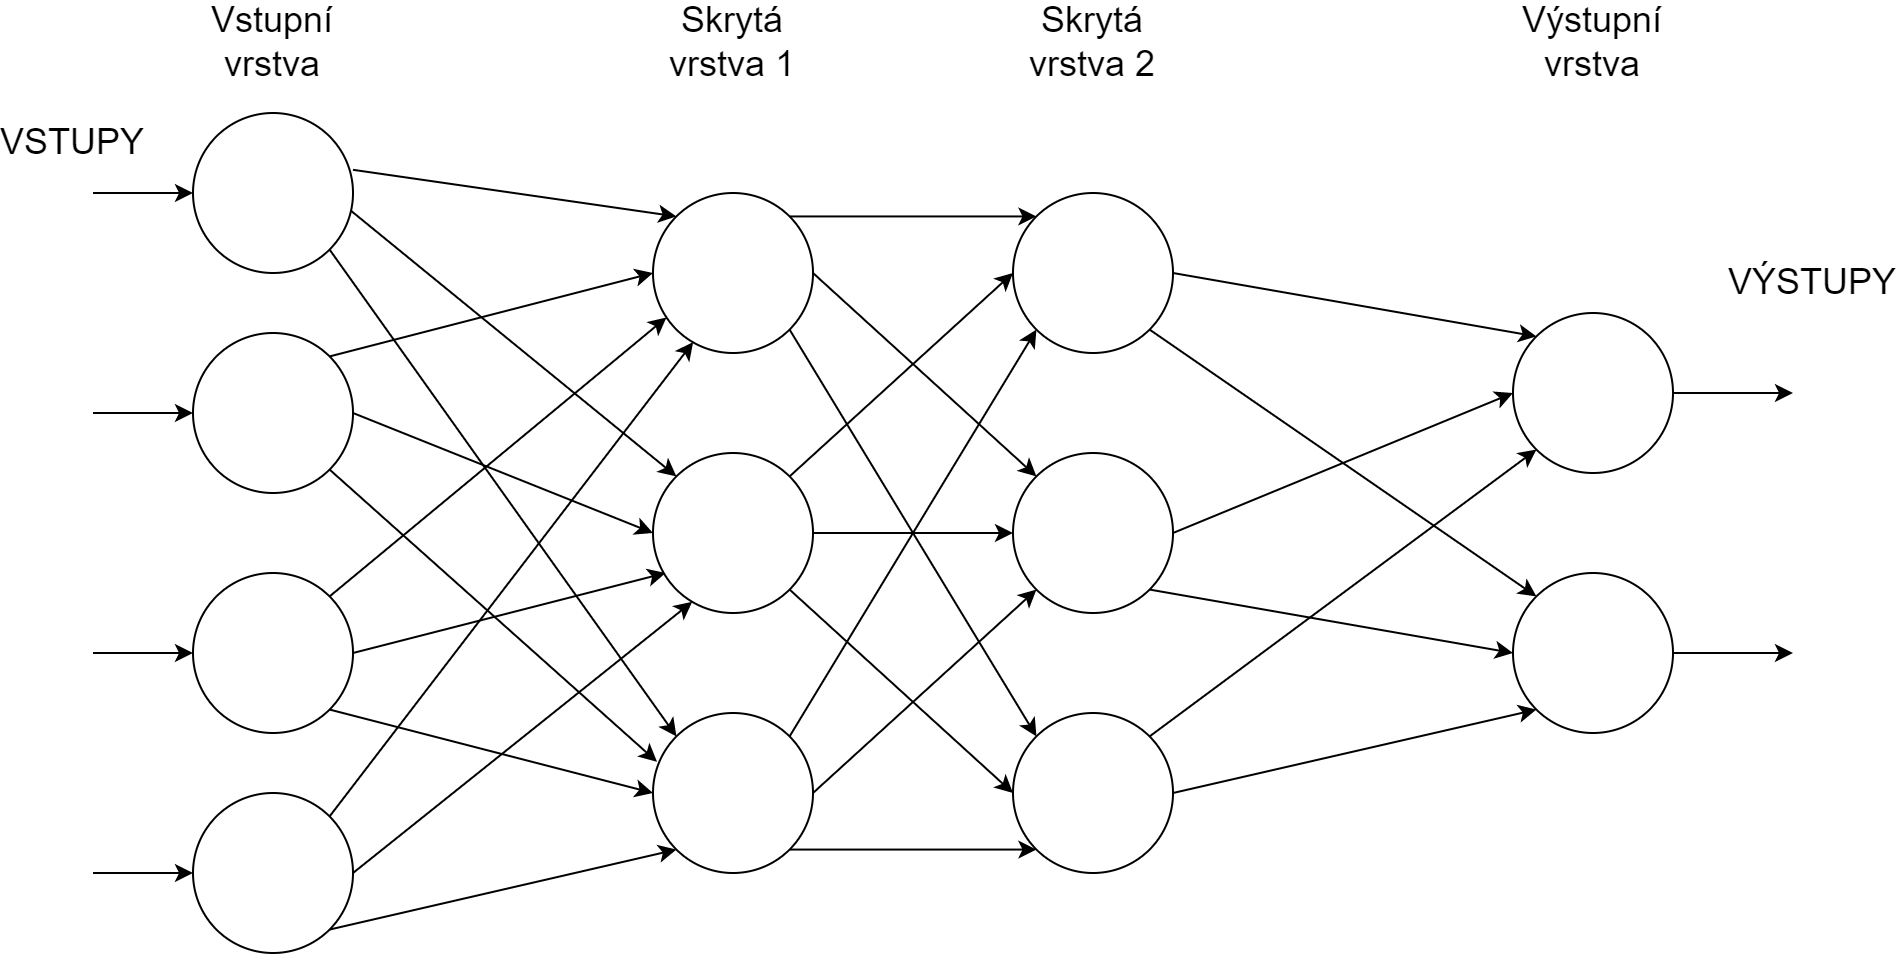
\includegraphics{obrazky-figures/nsexample.png}}
  \label{obrazek:nsexample}
  \caption{Propojení vrstev neuronů do neuronové sítě}
  \end{center}
\end{figure}

\subsection*{Učení}
Aby neuronová síť mohla fungovat, musí se natrénovat (tzn. nastavit co nejpřesněji váhy na vstupech neuronů). K~trénování se používají data z~datasetů (viz sekce \ref{sekce:datasety}). Trénování neuronových sítí lze rozdělit do 3 kategorií \cite{deeplearningbook}:

\begin{itemize}
  \item \textbf{Učení bez učitele} (anglicky unsupervised learning) -- tyto algoritmy procházejí data z~datasetu a provádějí nad nimi shlukování do tzv. clusterů.
  \item \textbf{Učení s~učitelem} (anglicky supervised learning) -- každým datům z~datasetu je přiřazena informace o~požadpvaném výstupu. Vstupy jsou zpracovány neuronovou sítí a podle chyby (rozdílu vstup/výstup) jsou upraveny parametry v~neuronové síti.
  \item \textbf{Posilované učení} (anglicky reinforcement learning) -- tento druh učení není vázán pouze na data z~datasetu, ale navíc interaguje s~prostředím.
\end{itemize}

\subsection*{Chyby}
Abychom byli schopní aktualizovat váhy vstupů jednotlivých neuronů, je potřeba měřit chybovost výstupu neuronové sítě. Jednou z~možností měření chyby (využitelné například při lineární regresi) je \emph{mean squared error}. Dle vztahu \ref{vzorec:mse} je vypočítána chybovost a jsou upraveny váhy. Snahou je chybu co nejvíce zmenšit.

\begin{equation}
  \label{vzorec:mse}
  MSE = \frac{1}{N} \sum_{i}^{N} (vystupNS - spravnyVystup)^2
\end{equation}

Při trénování může dojít k~situaci, kdy neuronová síť zvládá zpracovávat trénovací data s~velmi vysokou přesností, ale při použití testovacích (validačních) dat se chybovost zvyšuje. V~takovémto případě mluvíme o~\textbf{přetrénování} (anglicky overfitting). Druhým nežádoucím jevem, který může nastat je \textbf{nedotrénovanost} (anglicky underfitting) -- síť není dostatečně natrénovaná a dochází tak k~vysoké chybovosti (příčinou je například málo trénovacích dat).


\begin{figure}[H]
  \begin{center}
      \scalebox{0.18}{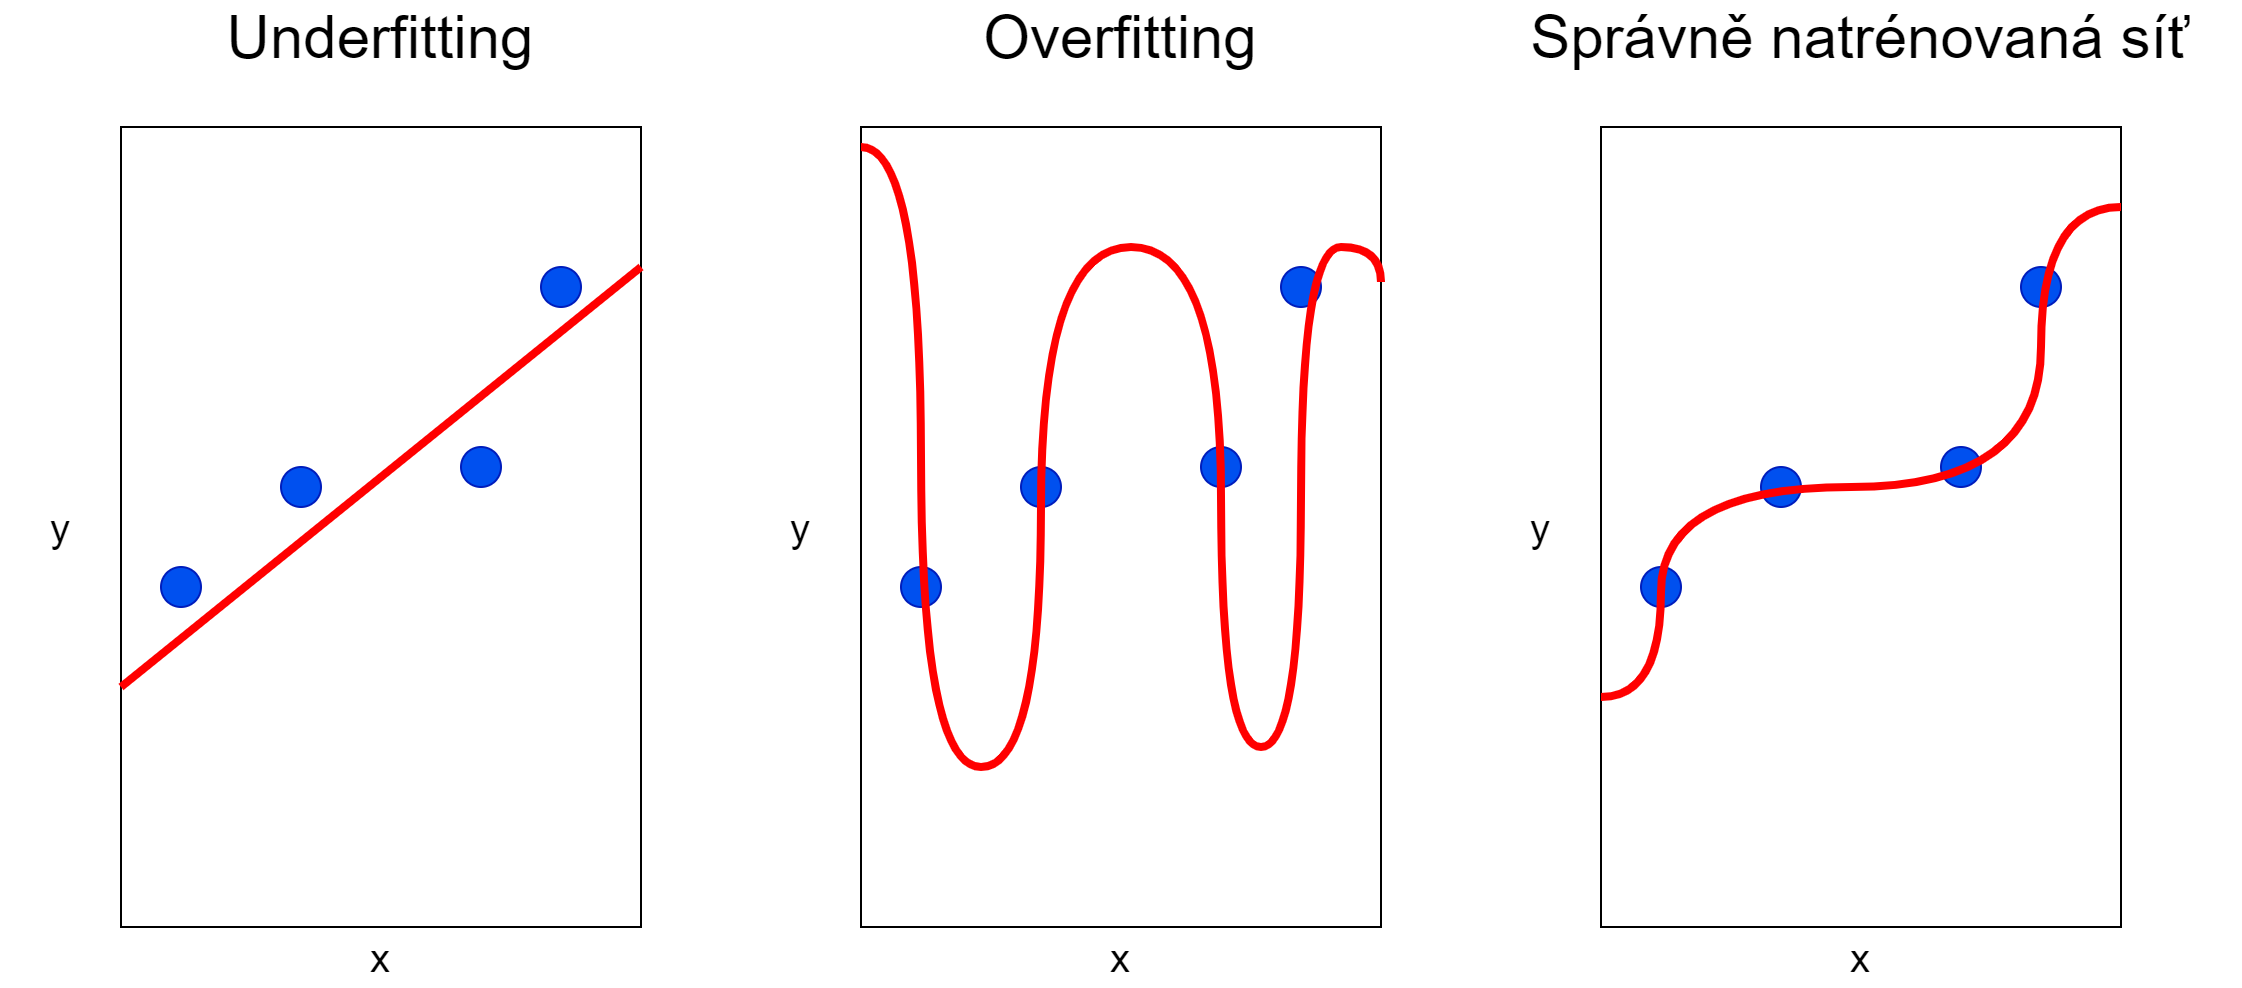
\includegraphics{obrazky-figures/fitting.png}}
  \label{obrazek:fitting}
  \caption{Ukázka výstupu neuronové sítě při nedoučení, přeučení a dostatečně dobrém množství dat pro učení}
  \end{center}
\end{figure}


\section{Datasety}
\label{sekce:datasety}
Datasetem rozumíme soubor podobných dat (například obrázků obličejů, číslic, předmětů nebo textů). Pro detekci obličejů se využívají datasety obsahující fotografie a videa lidí z~veřejně dostupných zdrojů (internet, televize) nebo jsou datasety přímo účelně vytvářeny (fotografování lidí) a následně je možné si je koupit nebo stáhnout. Data v~datasetech je nutné tzv. anotovat (označit co na daném obrázku je). V~případě tváří se může jednat například o~věk osoby, pohlaví, rasu, aby bylo možné určit zda po klasifikaci neuronovou sítí výstup odpovídá požadovanému výsledku. Následující podsekce popisují datasety používané k~učení neuronových sítí pro detekci obličejů.

\subsection*{Datasety lidských obličejů}
Dataset \textbf{CelebFaces Attributes Dataset} (CelebA) \cite{celeba} obsahuje více než $200 000$ obrázků obličejů známých osobností. Obrázky obsahují fotografie pořízené z~různých úhlů a jsou velmi dobře anotovány. Tento dataset je volně přístupný pro nekomerční účely.

\begin{figure}[H]
  \begin{center}
      \scalebox{0.6}{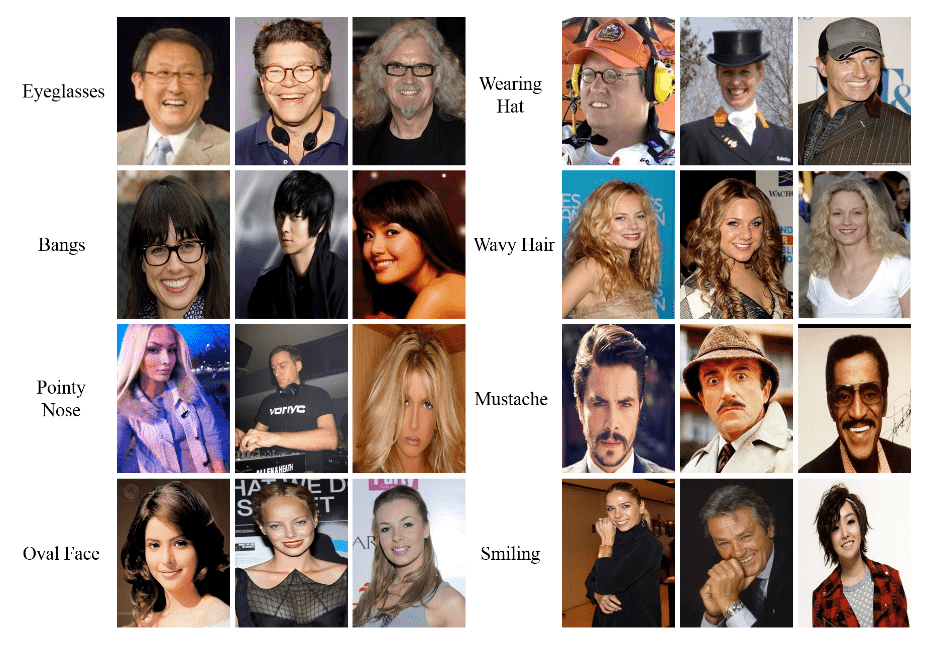
\includegraphics{obrazky-figures/celeba.png}}
  \label{obrazek:celeba}
  \caption{Příklady obličejů z~datasetu CelebA}
  \end{center}
\end{figure}

Dataset \textbf{DigiFace1M} \cite{digiface1m} se skládá z~1 milionu snímků digitálně vytvořených obličejů (viz obrázek \ref{obrazek:digiface}), čímž se vyhýbá případným právním a etnickým problémům, které mohou být spojeny s~využití tváří reálných osob. Při použití tohoto datasetu umělých tváří společně s~200 až 2000 fotografiemi tváří reálných lidí pro učení, lze dosáhnout podobných výsledků detekce jako s~datasety tvořenými čistě reálnými obličeji.

\begin{figure}[H]
  \begin{center}
      \scalebox{0.6}{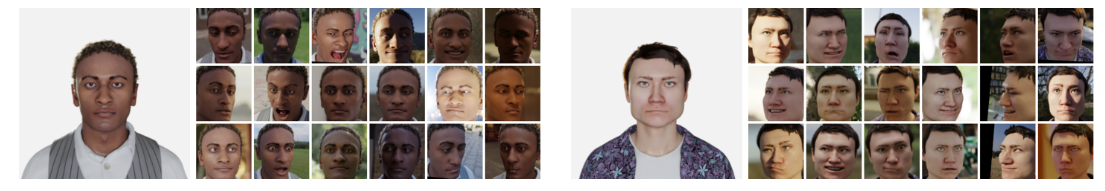
\includegraphics{obrazky-figures/digiface.png}}
  \label{obrazek:digiface}
  \caption{Příklady vygenerovaných obličejů pod různými úhly a různým osvětlením z~datasetu DigiFace1M \cite{digiface1m}}
  \end{center}
\end{figure}

\textbf{Multi-PIE} \cite{multipie} je dataset zaměřený na fotografie obličejů pořízených za různých světelných podmínek a pod různými úhly. Obshauje přes 750000 snímků, které byly vytvořeny vyfotografováním 337 lidí po dobu několika měsíců. Tento dataset je placený.

Dataset \textbf{UTKFace} \cite{utkface} obsahuje přes 20000 fotek obličejů lidí různých věků, pohlaví a~ras z~různých úhlů a~za rozličných světelných podmínek. Dataset je volně dostupný pro nekomerční použití. Data jsou podrobně anotovány dle vzorce \texttt{[věk]\_[pohlaví]\_[rasa]\_
[datum a čas].jpg}, kde věk je v~rozmezí 0--116 let, pohlaví muž/žena, rasa je jedna z~výčtu běloch, černoch, asiat, ind, ostatní a datum a čas uchovává informaci o~okamžiku zařazení fotografie do datasetu.

Dataset \textbf{DARK FACE} \cite{darkFace} obsahuje 6000 fotografií různých prostředí s~lidmi, pořízených za špatných světelných podmínek. Používá se mj.při hodnocení účinnosti detektorů obličejů. Dataset obsahuje jak anotované tak neanotované obrázky.

\section{Detektory obličeje}
\label{sekce:NSdetektory}

Jak již bylo zmíněno, detekce obličeje je jak samostatnou disciplínou, tak i vstupním bodem několika dalších analyzačních úkonů (rozpoznávání tváře, ověřování pomocí obličejů nebo identifikace obličejů). Zpracovávaný obrázek bývá rozdělen na několik menších oblastí (výřezů) a tyto výřezy bývají zpracovávány jednotlivě. 
Existuje řada různých druhů a architektur neuronových sítí využívaných k~detekci obličejů \cite{fdReviewNS}. Patří mezi ně například:

\begin{itemize}
  \item \textbf{Rotation invariant neural network} (RINN, rotačně invariantní neuronová síť) -- dokáže detekovat obličeje bez ohledu na úhel natočení tváře (není nutná normalizace v~preprocessingu). Systém tohoto typu neuronové sítě obsahuje několik sítí, s~tím že první se nazývá \emph{router network}. Tato síť určuje orientaci (natočení) výřezu obrázku a~připravuje (normalizuje) tak výřez pro 1 či více detekčních sítí.
  \item \textbf{Fast neural network} (FNN, rychlá neuronová síť) -- obrázek je rozdělen na malé podobrázky a každý podobrázek je zvlášť otestován na výskyt tváře rychlou neuronovou sítí. Cílem je snížení výpočetního času nutného pro nalezení obličeje.
  \item \textbf{Polynomial neural network} (PNN, polynomiální neuronová síť) -- oblasti v~obrázku jsou klasifikovány jako tvář/ne--tvář pomocí binomické projekce této oblasti do podprostoru vlastností obličeje naučeného tzv. základní analýzou komponent (anglicky principal component analysis, PCA). Zkoumáním vlivu PCA na vzorky lze detekovat zda se jedná o~obličej.
  \item \textbf{Convolutional neural network} (CNN, konvoluční neuronové sítě) -- samostatně popsány v~další podsekci. 
\end{itemize}


\subsection*{Konvoluční neuronové sítě}
Konvoluční neuronové sítě (CNN) \cite{cnnNlp, cnnCv, cnnIntro} jsou použity ve většině systémů v~oblasti počítačového vidění. Jelikož můžeme hodnoty pixelů vyjádřit čísly (používá se šedotónová varianta obrázku $\rightarrow$ při 8 bitové barevné hloubce může pixel nabývat hodnot 0 -- 255), lze tyto čísla použít jako vstupy neuronové sítě. Při vysokém rozlišení obrázku však nastává problém. Pokud bychom chtěli každou hodnotu pixelu použít na vstupu neuronové sítě pro celý obrázek naráz, měla by neuronová síť již u~obrázku s~rozměry 500 $\times$ 500 pixelů celkem 25000 vstupní neuronů, což je příliš výpočetně náročné. Proto se využívá konvoluce.

\textbf{Konvoluce} je okenní matematická funkce, při níž je na každou část obrázku (okno, \emph{window}) násobením aplikována matice (filtr, kernel, konvoluční jádro). Princip konvoluce zachycuje následující obrázek.

\begin{figure}[H]
  \begin{center}
      \scalebox{0.25}{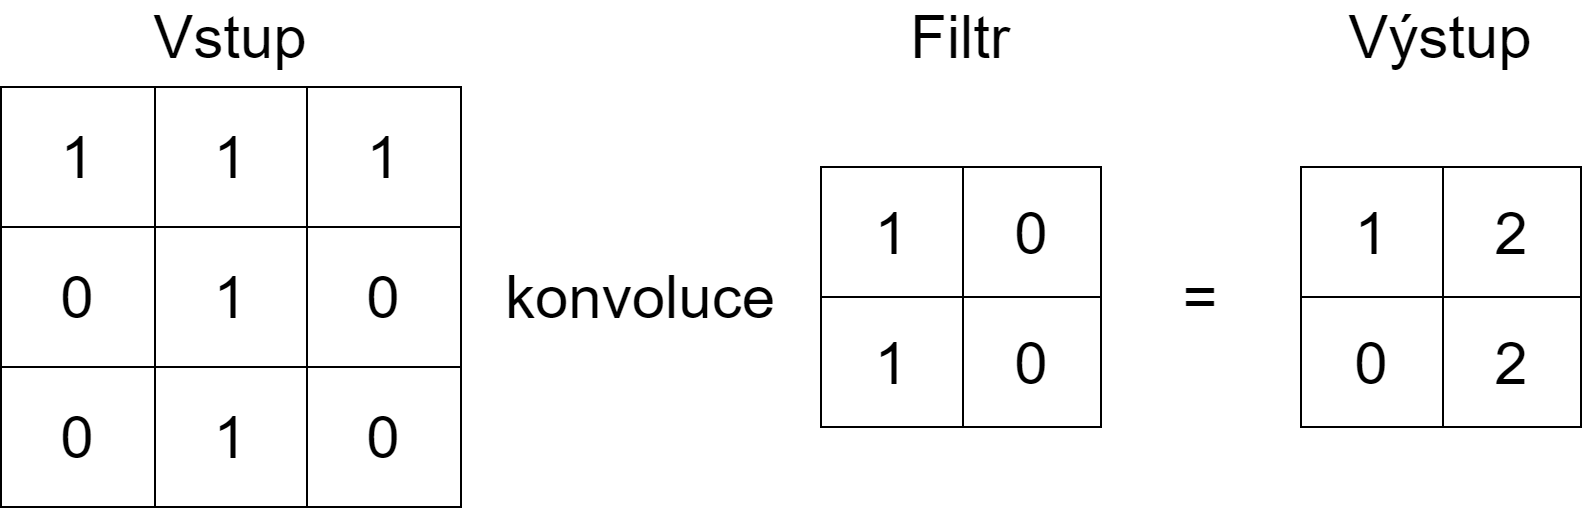
\includegraphics{obrazky-figures/principkonvoluce.png}}
  \label{obrazek:principkonvoluce}
  \caption{Princip konvoluce 2D obrázku s~rozměry 3$\times$3 a filtru $2\times2$}
  \end{center}
\end{figure}

Konvoluce dovoluje zásadně snížit počet nutných vstupů neuronové sítě. Navíc jsou konvoluční operace rychlé, protože tato funkce je hardwarově implementována na grafické kartě.

Jak lze vidět na obrázku \ref{obrazek:cnnpipeline} konvoluční neuronová síť se skládá z~několika vrstev.

\begin{figure}[H]
  \begin{center}
      \scalebox{0.55}{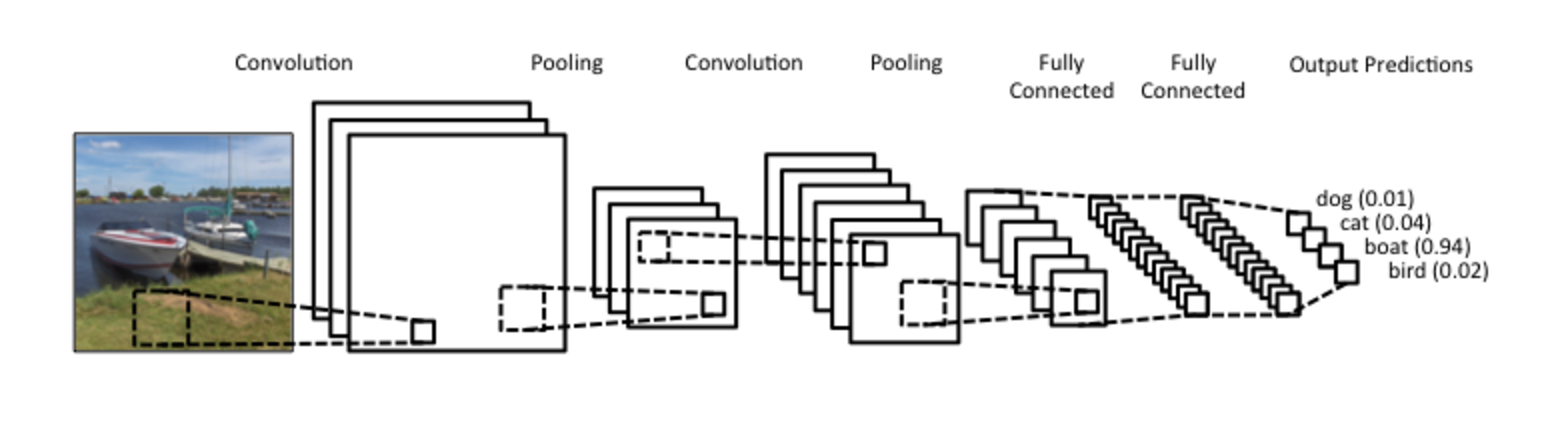
\includegraphics{obrazky-figures/cnnpipeline.png}}
  \label{obrazek:cnnpipeline}
  \caption{Řetězec vrstev konvoluční neuronové sítě \cite{cnnNlp}}
  \end{center}
\end{figure}

\textbf{Konvoluční vrstva} provádí výše popsanou konvoluci. Otázkou zůstává jak zpracovávat okraje obrázku. Existují dva přístupy:

\begin{itemize}
  \item \emph{Wide convolution} -- přidání nul kolem dokola obrázku a provedení konvoluce krajních hodnot (výstup bude stejně velký jako vstup).
  \item \emph{Narrow convolution} -- provedení konvoluce jako na obrázku \ref{obrazek:principkonvoluce}. Dojde ke zmenšení velikosti na výstupu.
\end{itemize}

Dalším parametrem konvolučních neuronových sítí je tzv. \textbf{stride} velikost. Určuje o~kolik hodnot se konvoluční jádro posune při každém kroku. Na obrázku \ref{obrazek:principkonvoluce} je použit stride 1. Větší hodnota stride vede k~menšímu výstupu. Běžně se používají hodnoty 1 nebo 2.

\textbf{Poolingová vrstva} (anglicky pooling layer) je vrstva aplikovaná po konvoluční vrstvě. Používá se ke snížení výpočetní náročnosti. Tím, že je aplikována statistická funkce (maximum, průměr) na výstup konvoluční vrstvy (většinou filtrem o~velikosti 2 $\times$ 2 se stride = 2), dojde ke zredukování počtu hodnot výsledné matice (viz obrázek \ref{obrazek:cnnpooling}).

\begin{figure}[H]
  \begin{center}
      \scalebox{0.25}{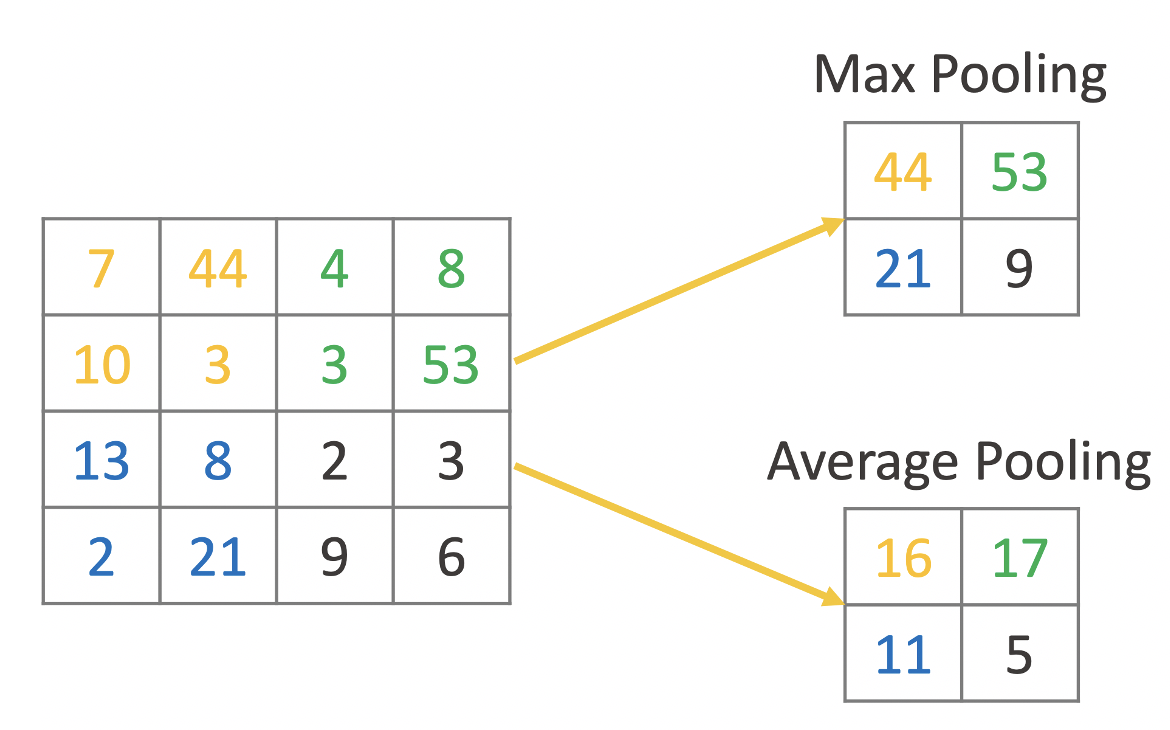
\includegraphics{obrazky-figures/cnnpooling.png}}
  \label{obrazek:cnnpooling}
  \caption{Řetězec vrstev konvoluční neuronové sítě \cite{cnnCv}}
  \end{center}
\end{figure}

V~reálné aplikaci jsou konvoluční a poolingové vrstvy poskládány za sebe. Na konci řetězce (obrázek \ref{obrazek:cnnpipeline}) se pak nachází část plně propojených vrstev neuronů (fully--conected layer).

\subsection*{Detektory}
Tato část popisuje vybrané existující detektory obličejů založené na neuronových sítí a provnání úspěšnosti detekce těchto detektorů s~detektory popsanými v~sekci \ref{sekce:detektory_bez_neuronovych_siti}.

\textbf{MTCNN} (Multi-Task Cascaded Convolutional Network) \cite{fdCNNComparison, MTCNN} provádí detekci obličejů pomocí kaskády konvoluční neuronových sítí. Algoritmus má dvě části. První část vytváří několik verzí vstupních obrázků, každa taková verze má jiné rozlišení. Druhá část složená z~kaskády neuronových sítí se stará o~detekci obličeje v~různých verzích obrázku. Použití více verzí obrázku umožňuje zvýšit efektivitu detekce.

Single shot detector \textbf{SSD} \cite{ssd} je konvoluční neuronová síť opět složená ze 2 částí, sloužící obecně k~detekci objektů. Tyto části jsou: a) natrénovaný detekční model (VGG--16 nebo jiný) a b) část SSD -- další konvoluční vrstva, která rozděluje obrázek pomocí mřížky (\emph{grid}) s~rozměry 4 $\times$ 4 nebo 8 $\times$ 8. V~každém takto vytvořeném bloku je pak hledán objekt (obličej).

Již výše zmíněný detekční/rozpoznávací algoritmus/neuronová síť \textbf{VGG--16} \cite{vgg-16} používá k~detekci konvoluční filtry o~rozměrech $3 \times 3$ v~několika konvolučních vrstvách za sebou (počet filtrů se s~každou další vrstvou navyšuje). Používá se zde stride o~hodnotě 1.

Detekční model \textbf{RetinaFace} \cite{lowLightFdReview} používá multitasking pro učení. Detekce probíhá určením pozice obličeje podle vyhledání pixelů, které tvář obsahuje. Model má 2 struktury: \emph{Multi--task loss} -- minimalizace chyb modelu a \emph{Dense Regression Branch} -- renderer, který filtruje obličeje a získává pixely z~vyrenderovaných obličejů.

\textbf{YOLO} (You Only Look Once) \cite{yolo} je stejně jako SSD tzv. single shot detektor -- rozděluje vstupní obrázek do mřížky a provádí detekci případně rekognici nad jednotlivými bloky mřížky. Pro každý blok je určena hodnota jistoty výskytu objektu. Na vstupu sítě YOLO jsou barevné obrázky o~velikosti 448 $\times$ 448 pixelů. Architektura neuronové sítě je složena ze 7 konvolučních vrstev následovaných pooling vrstvami a 3 plně propojenými vrstvami na výstupu.
YOLO má několik verzí, které se liší složením neuronové sítě a úspěšností detekce.

\subsection*{Porovnání výkonnosti detektorů}
Práce \cite{fdCNNComparison} se zabývá porovnáním detektorů Viola--Jones, Histogram of Oriented Gradients ze sekce \ref{sekce:detektory_bez_neuronovych_siti} a algoritmů založených na konvolučních neuronových sítích MTCNN a SSD (detektor VGG--16 je nahrazen detektorem MobileNet) ze sekce \ref{sekce:NSdetektory}. Testování bylo prováděno na datasetech AFW a WIDER FACE. Co se týká úspěšnosti detekce, nejlépe vyšel z~testu detektor MTCNN, nejrychlejší pak byl detektor SSD (viz obrázek \ref{obrazek:cnncomparison}). Z~detektorů založených na klasických metodách měl vyšší úspěšnost HOG, rychlejší však byl detektor Viola--Jones. Hodnota AP (average precision) udává průměrnou přesnost detekce a hodnota FPS (frames per second) počet snímků zpracovaných za sekundu.

\begin{figure}[H]
  \begin{center}
      \scalebox{0.7}{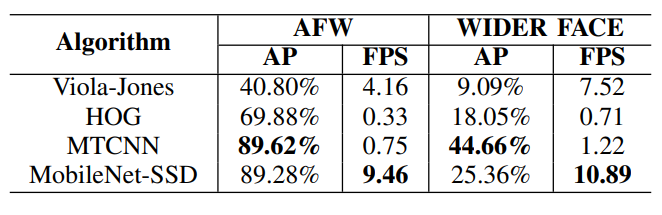
\includegraphics{obrazky-figures/cnncomparison.png}}
  \label{obrazek:cnncomparison}
  \caption{Výsledek testování detekčních algotitmů \cite{fdCNNComparison}.}
  \end{center}
\end{figure}

\subsection*{Detektory zaměřující se na špatné světelené podmínky}
Detektory zaměřující se na detekci ve špatných světelných podmínkách jsou buď specializované detektory, kdy je neuronová síť detektoru učena na datasetu vhodných obrázků (obrázky pořízené za špatných světelných podmínek) nebo je použit detektor obličeje natrénovaný na obyčejných snímcích. V~obou případech je nutno nejprve provést \emph{low--light image enhacement} (vylepšení obrázku) a~až poté přejít k~detekci.

Pro vylepšení obrázku existují různé metody \cite{lowLightFdReview}:
\begin{itemize}
  \item Mirnet,
  \item Adaptive Gamma Correction (AGC),
  \item Retinex,
  \item RetinexNet,
  \item a další.
\end{itemize}

\textbf{Mirnet} je metoda postavená na konvolučních neuronových sítí a jejím cílem je zvýšení kvality obrazu pomocí několika úprav v~konvolučních vrstvách.

\textbf{AGC} je metodou využívající gamma korekci k~vylepšení nasvícení scény (obrázku). Metoda navíc rozděluje obrázky podle intenzity gamma na tmavé (hodnota pod $0,5$) a světlé (hodnota nad $0,5$).

Koncept \textbf{Retinex} se snaží upravit kvalitu obrazu tak, aby odpovídala kvalitě lidského vidění. Dosaženo toho je tak, že je prováděno odmazávání odrazů světla z~obrázku.

\textbf{RetinexNet} vychází z~Retinexu a provádí dekompozici obrázku tak, aby došlo k~oddělení odrazů nezávislých na osvětlení a osvětlení se známou strukturou. Metoda také celkově upravuje nasvícení pro dosažení co největší konzistence světla v~obrázku.

Pro porovnání účinnosti \emph{image enhacement} metod lze použít 2 veličiny. \emph{Peak signal--noise ratio} (PSNR)-- poměr užitečného signálu k~šumu a~\emph{Structural similarity} (SSIM) -- index podobnosti 2 obrazů.

\begin{figure}[H]
  \begin{center}
      \scalebox{0.45}{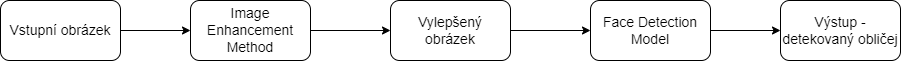
\includegraphics{obrazky-figures/iepostup.png}}
  \label{obrazek:iepostup}
  \caption{Řetězec postupu detekce obličeje ve zhoršených světelných podmínkách. Vychází z~\cite{lowLightFdReview}.}
  \end{center}
\end{figure}

Obrázek \ref{obrazek:iepostup}, který vychází ze článku \cite{lowLightFdReview} popisuje potřebný postup pro úpravu obrázku (preprocessing) a následné kroky vedoucí k~detekci obličeje. V~rámci tohoto článku jsou zpracovány výsledky detekce pomocí výše zmíněných metod vylepšení obrazu a detektoru RetinaFace (viz sekce Detektory). Jako testovací dataset byl použit dataset DARK FACE, popsaný v~sekci \ref{sekce:datasety}. V~rámci testování preprocessingových metod vylepšení obrazu bylo zjištěno, že nejlepší hodnoty PSNR ($19,48\:dB$) a SSIM ($0,74$) dosahuje metoda Mirnet (hodnoty dalších metod viz obrázek \ref{obrazek:psnrssim}).

\begin{figure}[H]
  \begin{center}
      \scalebox{0.7}{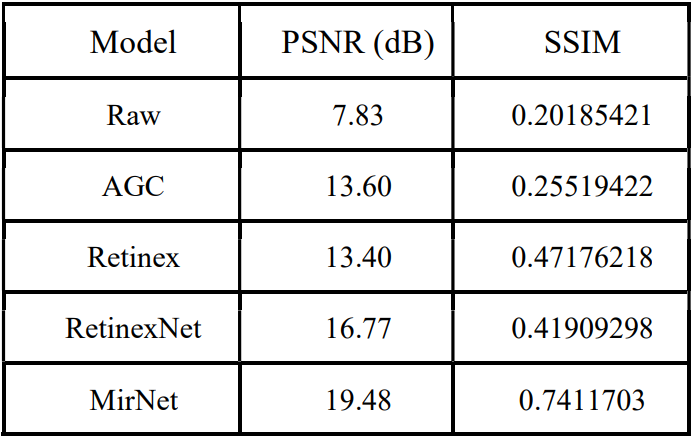
\includegraphics{obrazky-figures/psnrssim.png}}
  \label{obrazek:psnrssim}
  \caption{Hodnoty PSNR a SSIM pro metody vylepšení obrazu \cite{lowLightFdReview}.}
  \end{center}
\end{figure}

Výsledky detekce však ukázaly, že v~detekci obličejů si nejlépe vedl Retinex s~$0,43\:\%\:mAP$ (mean average precision -- průměrná přesnost detekce). Z~toho vyplývá, že lepší preprocessingová metoda nutně neznamená úspěšnější detektor.

Detekcí ve špatných světelných podmínkách se zabývá také článek \cite{HLAFace}. V~rámci tohoto článku byl vytvořen samoučící se (self--supervised) detektor dosahující $44,4\:\%\:mAP$ také na datech z~datasetu DARK FACE.

Práce \cite{fdExtremelyLowConditions} se rovněž zabývá detekcí nad datasetem DARK FACE při špatném osvětlení. Navržený algoritmus dosahuje $82,3\:\%\:mAP$. Algoritmus využívá 3 hlavní části umožňující dosáhnutí takto vysoké přesnosti detekce. Jsou to: \emph{Multi--scale retinex with color restoration} -- metoda podobná Retinexu, ale zachovává konzistenci barev, architektura konvolučních vrstev \emph{PyramidBox} a~\emph{Multi--scale test module} -- úpravy velikosti vstupního obrázku pro lepší detekci.

Velké rozdíly v~hodnotách $mAP$ jsou způsobeny tím, že neuronové sítě z~prací \cite{HLAFace, fdExtremelyLowConditions} jsou trénovány přímo na datasetu obličejů ve zhoršených pozorovacích podmínkách (specializoavné detektory), zatímco \cite{lowLightFdReview} používá model učený na běžných snímcích tváří.

\section{Frameworky pro neuronové sítě}
\label{sekce:frameworky_pro_ns}
Při programování neuronových sítí nebo obecně aplikací strojového učení se využívají k~tomu určené frameworky. Každý framework je trochu jiný a používá se k~jiným účelům. Všechny zde zmíněné frameworky podporují programovací jazyk Python. Mezi nejpoužívanější frameworky patří: TensorFlow, PyTorch, Keras, ONNX, Caffe \cite{nsFrameworks}.

\vspace{1em}
\textbf{TensorFlow} je framework pro jazyky R, C++, Python a další. Má několik modulů s~rozličnými funkcionalitami. Je velmi rozšířený a implementuje jej například Google překladač. Dokumentace je velmi podrobná a framework podporuje paralelismus napříč GPU.

\textbf{PyTorch} je vědecký framework použitelný v~jazyce Python, vhodný na prototypování. Navíc podporuje GPU paralelismus.

Dalším frameworkem je \textbf{Keras}, v~němž se programují konvoluční a rekurentní neuronové sítě. Je minimalistický a snadno se integruje spolu s~TensorFlow.

Framework \textbf{ONNX} je open source framework pro hluboké učení. Modely vytvořené v~ONNX lze konvertovat do jiných frameworků (TensorFlow, Keras).

\textbf{Caffe} je framework podporovaný napříč různými programovacími jazyky (C, C++, Python, MATLAB) a je vhodný pro konvoluční neuronové sítě. Umožňuje nastavit parametry sítě a natrénovat síť, není nutné ji přímo vytvářet.

V~rámci této práce jsou použity frameworky TensorFlow a Keras. 


%%%%%%%%%%%%%%%%%%%%%%%%%%%%%%%%%%%%%%%%%%%%%%%%%%%%%%%%%
%       KAPITOLA 4 - Systémy pro detekci a akcelerace detekce
%%%%%%%%%%%%%%%%%%%%%%%%%%%%%%%%%%%%%%%%%%%%%%%%%%%%%%%%%
\chapter{Systémy pro detekci obličejů a~akcelerace detekce}
\label{kapitola:kamery_a_systemy}
Detekci obličejů s~využitím počítačových programů lze provádět nad snímkem 
(fotografií, obrázkem), sadou snímků,
videozáznamem nebo tzv. real\,--\,timově pomocí kamer a kamerových systémů.
V~této kapitole jsou popsány aktuálně využívané prostředky pro vytváření 
obrázků k~detekci obličejů (kamery) a také dostupná řešení zabývající se 
detekcí, a to jak placené komerční, tak neplacené open--source systémy.

\section{Kamery}
Nezbytnou součástí oboru detekce obličejů jsou kamery a kamerové systémy.
Existují kamery specializované k~detekci či rozpoznávání obličejů 
a kamery obyčejné, které pouze zprostředkovávají obraz dále ke zpracování.

Specializované kamery se používají například k~zabezpečení objektů nebo
jako domovní videozvonky, kdy kamera (respektive její software) v~zachyceném
obraze detekuje a rozpozná obličej, a následně může vykonat přiřazenou akci 
(spustit alarm, poslat notifikaci, umožnit osobě vstup...) \cite{securityCamsWeb}.

Další oblastí, kde se kamery s~detekcí a rozpoznáváním obličejů uplatní je
bezesporu dohled ve veřejných prostorech (anglicky CCTV surveillance). 
Detekce obličeje může sloužit k~hledání podezřelých osob v~záznamech z~dohledových
kamer. Tyto záznamy jsou shromážďovány na serveru, pomocí detekce jsou
z~obrazu vyřezány fragmenty s~obličeji lidí a poté jsou tyto fragmenty
porovnány rozpoznávacím algoritmem s~obličeji hledaných osob. Při shodě
dochází k~informování administrátora systému, který podnikne další kroky 
\cite{suspectIdentification}. 

Kamery tedy mají v~doméně detekce obličejů nezastupitelnou roli, na 
jejich praktické využití v~systémech a řešení pro detekci se zaměřuje následujících
podkapitola.

\section{Dostupná řešení}
Řešení umožňující detekci (a často i rekognici) obličejů lze rozdělit do dvou kategorií: 
komerční (placené, profesionální) a nekomerční (zdarma, open--source, amatérské).
V~následujících dvou podsekcích jsou popsány konkrétní systémy umožňující
detekci obličejů včetně jejich výhod a nevýhod.

\subsection*{Komerční}
Komerčně využívaná zařízení pro detekci, případně rekognici lze běžně zakoupit 
a používat ve firemním nebo domácím prostředí. Mezi zástupce těchto zařízení
patří například produkty firem Netatmo, Google, Nest \cite{securityCamsWeb2}.

\begin{figure}[H]
  \begin{center}
      \scalebox{0.5}{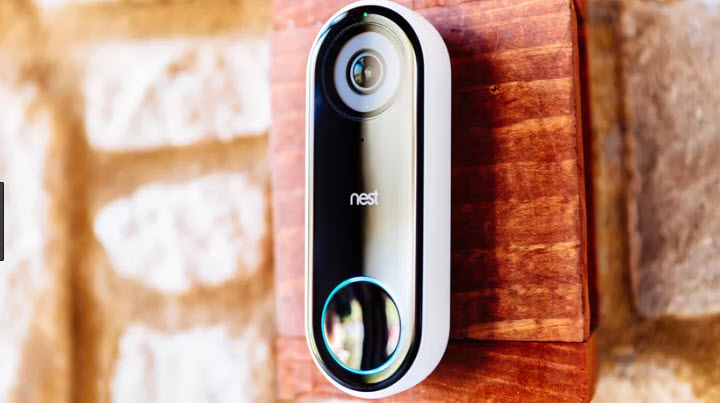
\includegraphics{obrazky-figures/nest-hello.png}}
  \label{nest}
  \caption{Nest Hello \cite{securityCamsWeb2}}
  \end{center}
\end{figure}

\subsection*{Nekomerční}
Nekomerční řešení pro detekci obličejů zahrnují frameworky s~otevřeným zdrojovým
kódem (open--source). Tyto frameworky a řešení využívají neuronové sítě, které jsou trénovány
pomocí datasetů a následně jsou využity k~detekci obličeje 
\cite{faceRecognitionFrameworks}.
Mezi open--source řešení patří například TinaFace \cite{TinaFace} nebo MTCNN \cite{MTCNN}, další volně použitelné frameworky popisuje sekce \ref{sekce:frameworky_pro_ns}.


\section{Akcelerace detekčních algoritmů}
\label{sekce:akcelerace}

S~rozmachem využívání strojového učení a neuronových sítí se objevila potřeba zrychlení těchto sítí. Proto byly vytvořeny specializované zařízení s~cílem urychlit výpočty a snížit energetickou náročnost výpočtů ve srovnání s~běžnými (univerzálními) výpočetním prostředky. Vznikly tak hardwarové akcelerátory neuronových sítí. Příkladem jsou Intel Neural Compute Stick 2 \cite{ncs2}, Coral \cite{coral} nebo Nvidia Jetson \cite{jetson}.

Existují různé typy architektur akcelerátorů \cite{acceleratorsSurvey}, mezi něž patří architektury popsané v~tomto odstavci.
\textbf{NPU} (neural processing unit) -- k~provádění matematických operací využívají speciální NPU obsahující PE (processing engines). NPU používá hardwarové verze MLP (multi--layer perceptron), pro dosažení zrychlení obecného výpočtu (nejen neuronových sítí). Pokud je část programu určená ke zrychlení spouštěna často a jsou dobře známy vstupy a výstupy, lze tuto část programu zrychlit pomocí NPU. Příkladem algoritmu pro zrychlení je rychlá Fourierova transformace (FFT).

Architektura \textbf{RENO} využívá memristory (ReRAM) -- speciální druh paměti jejíž struktura umožňuje urychlit maticové a vektorové násobení.

Mezi další akcelerátory patří série akcelerátorů \textbf{DianNao} využívaná na akademické půdě. Tyto akcelerátory obsahují NFU (neural functional unit), vstupní, výstupní a synaptický buffer a kontrolní procesor.

Průmyslovým akcelerátorem od Google je \textbf{TPU} (tensor processing unit). Je použitelný i přes cloud.

Kromě ReRAM jsou v~akcelerátor používány i paměti typu HMC (hybrid memory cube). Obě paměti (ReRAM a HMC) umožňují tzv. \emph{processing--in--memory}, takže snižují čas výpočtu tím, že není nutno data přesouvat mezi procesorem a pamětí. Příklady akcelerátorů postavených na HMC je Neurocube \cite{neurocube} nebo Tetris \cite{tetris}.

Většina akcelerátorů je zaměřena na výpočty s~již natrénovanou neuronovou sítí, jen pár jich podporuje učení neuronových sítí. V~některých případech (edge computing) se ke zrychlení neuronové sítě používají cloudové služby -- v~datacentrech provádějí náročné výpočty grafické karty a výsledky spolu s~nenáročnými výpočty jsou zpracovány například na IoT (Internet of Things -- internet věcí) nebo mobilních zařízeních.

\subsection*{Intel Neural Compute Stick 2}

Intel Neural Compute Stick 2 (NCS2) \cite{ncs2} (obrázek \ref{obrazek:ncs2}) je akcelerátor neuronových sítí zaměřený na počítačové vidění. Obsahuje VPU (vision processing unit) Intel Movidius X. Připojuje se k~počítači přes rozhraní USB 3.0 a umožňuje urychlení neuronové sítě bez použití cloudu a s~nízkými energetickými nároky (například v~kombinaci s~Raspberry Pi). Podporuje mj. frameworky TensorFlow, Caffe, PyTorch, Keras popsané v~sekci \ref{sekce:frameworky_pro_ns}. Pro práci s~NCS2 se používá knihovna/framework OpenVINO \cite{openvino}. 

\begin{figure}[H]
  \begin{center}
      \scalebox{0.25}{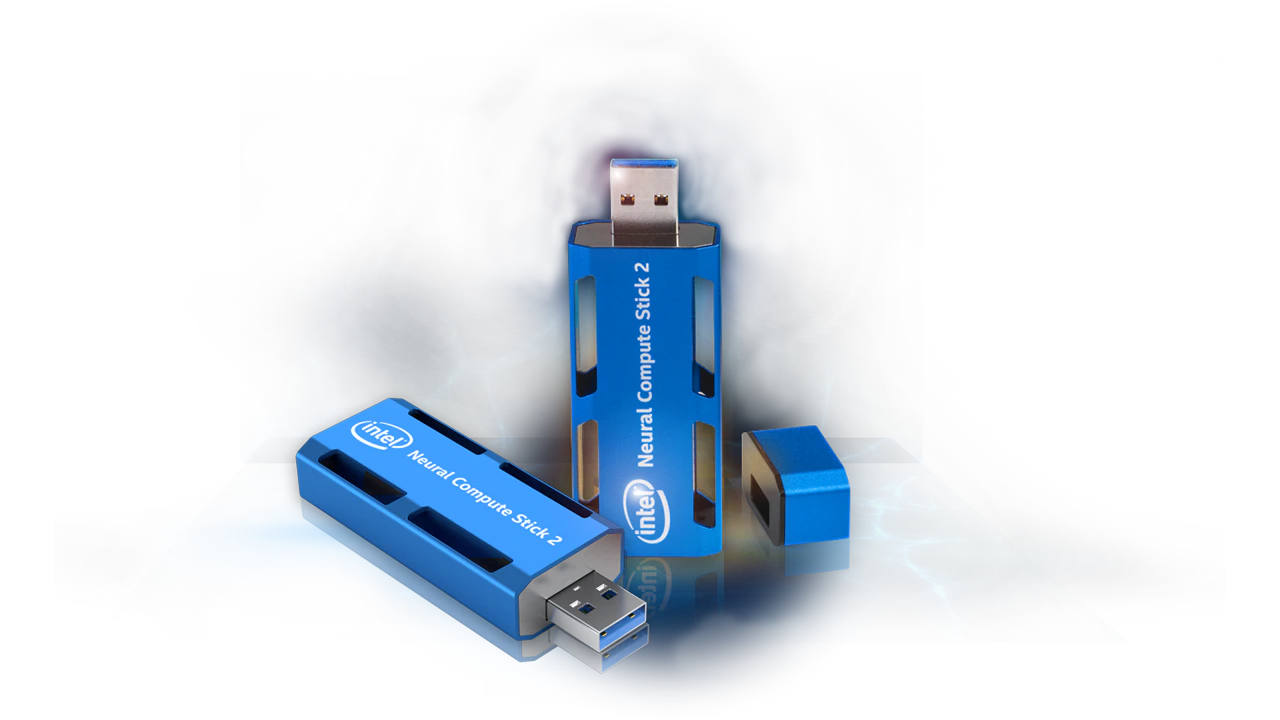
\includegraphics{obrazky-figures/ncs2.png}}
  \label{obrazek:ncs2}
  \caption{Intel Neural Compute Stick 2 \cite{ncs2}}
  \end{center}
\end{figure}

Experimenty provedené v~\cite{ncs2testYolo} porovnávají výkonnost akcelerátorů Nvidia Jetson Nano, Nvidia Jetson Xavier NX a Raspberry Pi 4B s~NCS2. K~porovnání posloužily frameworky YOLOv3 popsaný v~sekci \ref{sekce:NSdetektory} a YOLOv3--tiny. Experimenty byly založeny na detekci objektů ve dvou videích.
\begin{itemize}
  \item \emph{Video1} -- rozlišení 768 $\times$ 436 pixelů, celkem 1596 framů
  \item \emph{Video2} -- rozlišení 1920 $\times$ 1080 pixelů, celkem 960 framů 
\end{itemize}

Naměřené výsledky zobrazuje obrázek \ref{obrazek:ncs2test}.

\begin{figure}[H]
  \begin{center}
      \scalebox{0.5}{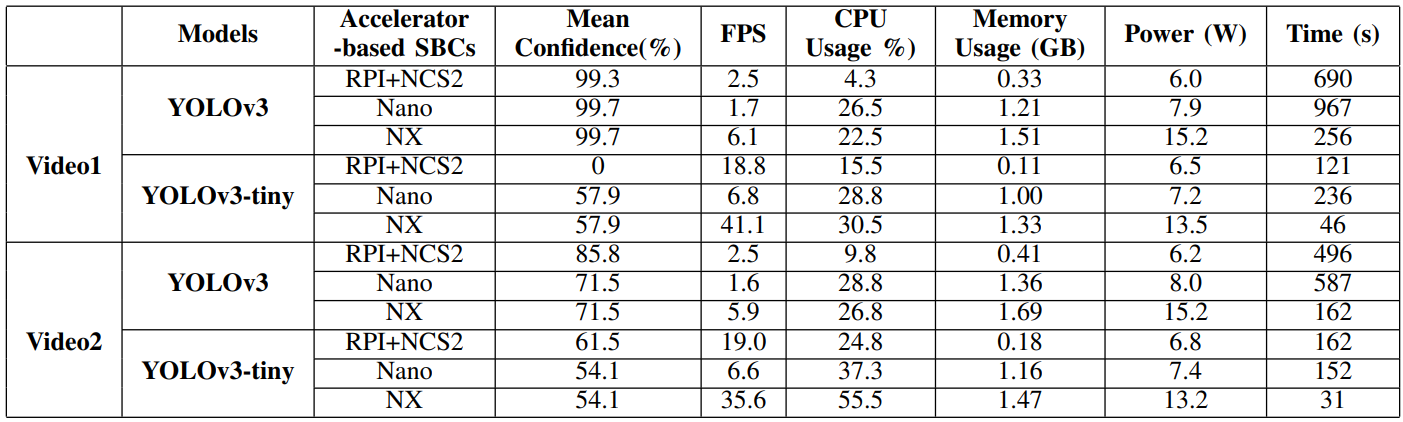
\includegraphics{obrazky-figures/ncs2test.png}}
  \label{obrazek:ncs2test}
  \caption{Výsledky testu akcelerátorů neuronovýxh sítí s~modelem YOLOv3 a~YOLOv3-tiny \cite{ncs2testYolo}}
  \end{center}
\end{figure}

Z~tabulky v~obrázku \ref{obrazek:ncs2test} můžeme vidět, že NCS2 dosahuje podobných výsledků detekce ve \emph{Videu1} jako Jetson Nano a zároveň nejméně zatěžuje procesor. U~\emph{Videa2} má NCS2 nejlepší výsledky detekce. Využití paměti s~větším vstupem roste, stále je však mezi konkurenty nejnižší, to samé lze řící o~spotřebě energie. S~dostatečně dobrým modelem neuronové sítě je tak NCS2 úsporným akcelerátorem s~vysokou úspěšností detekce.


\subsection*{OpenVINO}
Framework/knihovna OpenVINO se stará o~konverzi a optimalizaci natrénovaného modelu neuronové sítě v~jednom z~podporovaných frameworků (viz obrázek \ref{obrazek:ovchart}) pro použití na NCS2 nebo jiném zařízení (procesory, grafické karty). OpenVINO se nezaměřuje pouze na oblast počítačového vidění, ale na neuronové sítě obecně.

\begin{figure}[H]
  \begin{center}
      \scalebox{0.22}{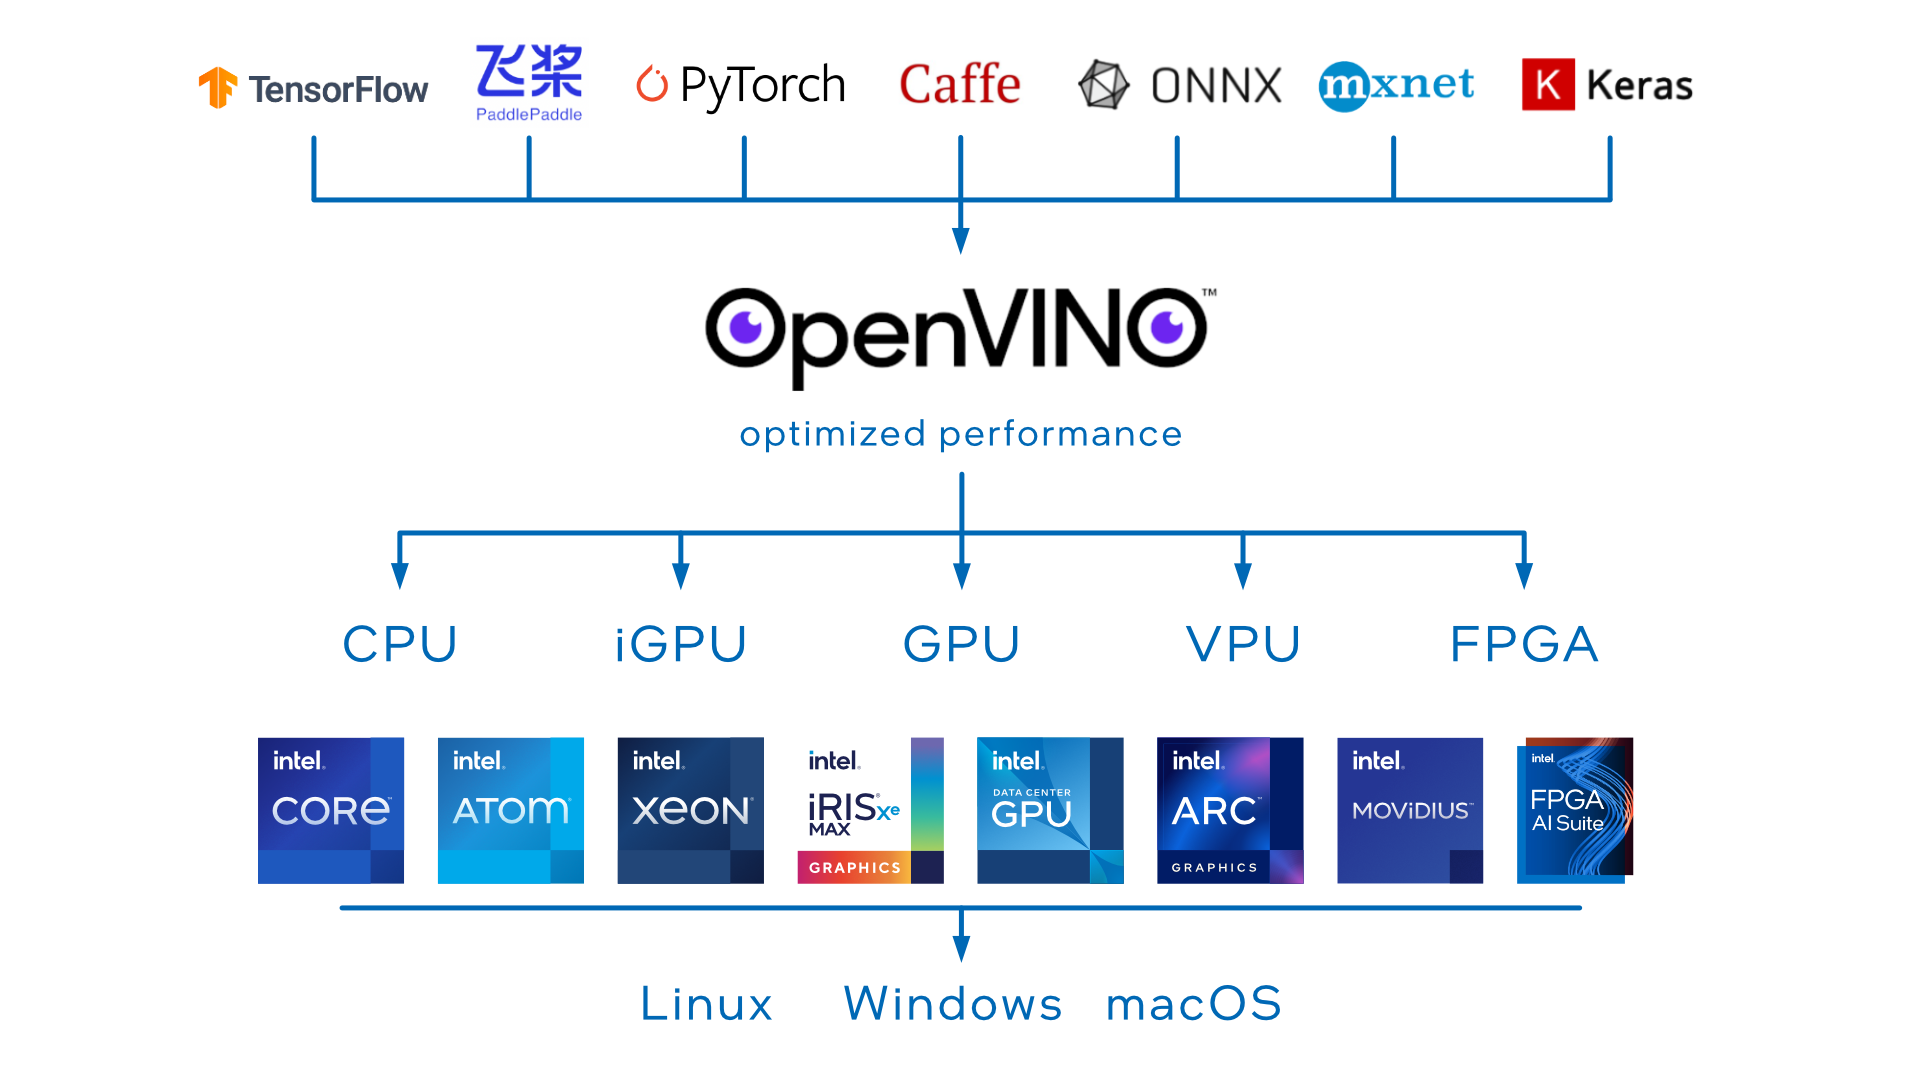
\includegraphics{obrazky-figures/ovchart.png}}
  \label{obrazek:ovchart}
  \caption{Využití frameworku OpenVINO \cite{openvino}}
  \end{center}
\end{figure}

%%%%%%%%%%%%%%%%%%%%%%%%%%%%%%%%%%%%%%%%%%%%%%%%%%%%%%%%%
%       KAPITOLA ZÁVĚR
%%%%%%%%%%%%%%%%%%%%%%%%%%%%%%%%%%%%%%%%%%%%%%%%%%%%%%%%%
\chapter{Závěr}
\label{kapitola:zaver}
V~rámci tohoto textu byla představena problematika detekce obličejů v~reálných podmínkách, dále byly popsány problémy omezující detekci a klasické algoritmy detekce obličejů. V~samostatných kapitolách a sekcích byly popsány neuronové sítě (obecně, konvoluční) a algortimy pro detekci založené na neuronových sítích. Dále pak existující komerční a nekomerční řešení a systémy detekce a možnosti akcelerace neuronových sítí specializovaným hardawarem.

V~této práci bude pokračováno návrhem neuronové sítě pro detekci ve špatných světelných podmínkách, návrhem Python aplikace, její implementací a provedením experimentů s~vytvořeným řešením a existujícími řešeními.